\documentclass[a4paper,11pt, oldfontcommands]{memoir}
%\documentclass[b5paper,10pt,twoside]{memoir}
% Ved a4 format skal nedenst�ende nok justeres en del
\setlrmarginsandblock{3.5cm}{2.5cm}{*}
\setulmarginsandblock{3cm}{*}{1.2}

% The following is needed in order to make the code .ps compatible
% with both latex/dvips and pdflatex.
\ifx\pdftexversion\undefined
	\usepackage[dvips]{graphicx}
\else
	\usepackage[pdftex]{graphicx}
	\DeclareGraphicsRule{*}{mps}{*}{}
\fi

\usepackage[retainorgcmds]{IEEEtrantools}
%\usepackage{graphicx}
\usepackage{pstricks,pst-node,pst-text,pst-3d}
\usepackage{marginnote}
\usepackage{array,booktabs,longtable}
\usepackage{url}
\usepackage{color}
\usepackage{array}
\usepackage[oldenum]{paralist}
\usepackage{enumitem}
\usepackage{wrapfig}
\usepackage{listings}
\usepackage{todonotes}


%\definecolor{webblue}{rgb}{0.0,0.05,0.45}
\definecolor{MyDarkBlue}{rgb}{0,0.08,0.45}
%\definecolor{webred}{rgb}{0.75,0,0}

\usepackage[T1]{fontenc}
\checkandfixthelayout
% ops�tning af pagestyles
\makepagestyle{book} % laver en ny tom pagestyle
\makeevenhead{book}{}{\small\sffamily\leftmark}{}
\makeoddhead{book}{}{\small\sffamily\rightmark}{}
\makeevenfoot{book}{\small\sffamily\thepage}{}{}
\makeoddfoot{book}{}{}{\small\sffamily\thepage}
\makeatletter

\makepsmarks{book}{%
\renewcommand\chaptermark[1]{%
\markboth{%
\ifnum \value{secnumdepth} > 1
\if@mainmatter % indenfor frontmatter er der intet kapitel nummer
\@chapapp\ \thechapter. \ % \@chapapp er lidt dum, se nedenfor
\fi
\fi
##1}{}}%
\renewcommand\tocmark{\markboth{\contentsname}{\contentsname}}%
\renewcommand\lofmark{\markboth{\listfigurename}{\listfigurename}}%
\renewcommand\lotmark{\markboth{\listtablename}{\listtablename}}%
\renewcommand\bibmark{\markboth{\bibname}{\bibname}}%
\renewcommand\indexmark{\markboth{\indexname}{\indexname}}%
\renewcommand\sectionmark[1]{\markright{##1}}%
\renewcommand\subsectionmark[1]{\markright{##1}}%
\renewcommand\subsubsectionmark[1]{\markright{##1}}%
}
\makeatother

\pagestyle{book}
% laver om p� plain stilen
\copypagestyle{plain}{book}
\makeevenhead{plain}{}{}{}
\makeoddhead{plain}{}{}{}

%**************** Headlines ****************************************************
% konfiguration af kapitel titel font samt fonte til sections
\renewcommand\chapnamefont{\Huge\bfseries\sffamily}
\renewcommand\chapnumfont{\chapnamefont}
%\renewcommand\chaptitlefont{\color{webred}\Huge\usefont{OT1}{phv}{bc}{n}\selectfont\raggedright}
\renewcommand\chaptitlefont{\Huge\usefont{OT1}{phv}{bc}{n}\selectfont\raggedright}
%\setsubsecheadstyle{\color{MyDarkBlue}\large\bfseries\sffamily\raggedright}
\setsubsecheadstyle{\large\bfseries\sffamily\raggedright}
%\setsubsubsecheadstyle{\color{webred}\Huge\usefont{OT1}{phv}{bc}{n}\selectfont\raggedright}
\setsubsubsecheadstyle{\Huge\usefont{OT1}{phv}{bc}{n}\selectfont\raggedright}
% Rule under headline.. (Underline section headlines med de 4 linier herunder) 
%\newcommand{\ruledsec}[1]{%
%\Large\usefont{OT1}{phv}{b}{n}\selectfont\raggedright #1 %\color{webred}\rule[15pt]{\textwidth}{1.0pt}} 
%\setsecheadstyle{\ruledsec} %ud-kommenter linie herunder
\setsecheadstyle{\Large\usefont{OT1}{phv}{b}{n}\selectfont\raggedright}

\usepackage{titlesec}
\usepackage{titletoc}
% Afstande mellem overskrifter og tekst
\titleformat{\subsection}
%{\color{MyDarkBlue}\usefont{OT1}{phv}{b}{n}\selectfont}{\thesubsection}{1em}{}
{\usefont{OT1}{phv}{b}{n}\selectfont}{\thesubsection}{1em}{}
\titleformat{\subsubsection}
%{\color{MyDarkBlue}\usefont{OT1}{phv}{b}{n}\selectfont}{\thesubsubsection}{1em}{}
{\color{black}\usefont{OT1}{phv}{b}{n}\selectfont}{\thesubsubsection}{1em}{}
\titlespacing{\subsection}{0pt}{15pt}{10pt}
\titlespacing{\subsubsection}{15pt}{15pt}{10pt}
\titlespacing{\section}{15pt}{35pt}{10pt}
%***********  section number in margin ****************************************
\makeatletter
\def\@seccntformat#1{\@ifundefined{#1@cntformat}%
{\csname the#1\endcsname\quad}% default
{\csname #1@cntformat\endcsname}% individual control
}
%\def\section@cntformat{\color{webred}\protect\makebox[0pt][r]{\thesection.\quad}}
\makeatother


% s�g for at hvis en \section el.lign. flyttes til en ny side
% da skal siden f�r ikke str�kkes
\raggedbottomsectiontrue
% justering af afsnitsnummerering og ToC dybde
\setsecnumdepth{subsubsection} % til og med
\maxsecnumdepth{subsubsection} % underligt koncept
%\settocdepth{subsection} %til og med
% nogle pakker man ofte anvender
\usepackage[ansinew]{inputenc} % eller ansinew hvis Windows
%*******************************************************************************
\usepackage[T1]{fontenc}
\usepackage{amsmath,amssymb}
\usepackage{mathtools}
\usepackage{graphicx}
\usepackage{fix-cm,fixltx2e}
\usepackage{soul}

\DeclareRobustCommand{\SetFourierSpace}{%
\fontdimen2\font=1.13\fontdimen2\font}
\sodef\an{}{0.13em}{0em}{0em} \sodef\ann{}{0.13em}{0.5em}{0em}
%******************************************************************************
\let\footruleskip\relax % for compatibility of memoir and fancyhdr
%% Use fancy chapter headers, with Jos Dingjan's modifications,
%% plus my own tweaks. This style is not part of teTeX,
%% so we are using a local (and renamed) copy. Reverted to original!
% \usepackage[Lenny]{fncychapleo}
\usepackage[Lenny]{fncychap}
\usepackage{fancyhdr}

% Setup af fncychap Lanny chapter header
\ChNameVar{\LARGE\usefont{OT1}{phv}{m}{n}\selectfont\raggedright}
\ChNumVar{\fontsize{75}{10}\usefont{OT1}{cmr}{m}{n}\selectfont\raggedright}
\ChTitleVar{\Huge\usefont{OT1}{phv}{bc}{n}\selectfont\raggedright}

%*******************************************************************************

\makeatletter
\newcommand\figcaption{\def\@captype{figure}\caption}
\newcommand\tabcaption{\def\@captype{table}\caption}
\makeatother

%\newenvironment{narrow}[2]{%
%\begin{list}{}{%
%\setlength{\topsep}{0pt}%
%\setlength{\leftmargin}{#1}%
%\setlength{\rightmargin}{#2}%
%\setlength{\listparindent}{\parindent}%
%\setlength{\itemindent}{\parindent}%
%\setlength{\parsep}{\parskip}}%
%\item[]}{\end{list}}

\newlength{\marginwidth}
\setlength{\marginwidth}{2.0\oddsidemargin} %bredden af billeder ud i margin'en

% Picture Handling
\usepackage{subfig}
\usepackage[leftcaption]{sidecap}
%\usepackage{varioref} %For smarte referencer med \vref istedet for \ref
\usepackage[hidelinks]{hyperref}
\usepackage{cleveref}
\usepackage{calc}% auto udregn

\usepackage{tikz}
\usepackage{pgf-umlsd}
\usepackage{tikz-uml}
\usepackage{pgfplots}
\pgfplotsset{compat=1.8}
\usepgfplotslibrary{statistics}
\usetikzlibrary{arrows, chains, graphs}

\graphicspath{{figures/}}
\sidecaptionvpos{figure}{t} %sidecaption aligned med toppen af billede
\usepackage{caption}
%\DeclareCaptionFont{red}{\color{webred}}
\DeclareCaptionFont{defaultCapFont}{\color{black}}
\captionsetup{singlelinecheck=false,font=footnotesize,labelfont={bf,defaultCapFont},format=hang}

\DeclareCaptionFormat{llap}{\llap{#1#2}#3\par}
\strictpagechecktrue
\makeatletter
\DeclareRobustCommand*{\bfseries}{%
  \not@math@alphabet\bfseries\mathbf
  \fontseries\bfdefault\selectfont
  \boldmath
}
\makeatother


% Added possibility for description refferences by using the \itemlabel{}{} command %
\makeatletter
\newcommand{\labitem}[2]{%
	\def\@itemlabel{''\textbf{#1}''}
	\item
	\def\@currentlabel{\textit{#1}}\label{#2}}
\makeatother
%%%%%%%%%%%%%%%%%%%%%%%%%%%%%%%%%%%%%%%%%%%%%%%%%%%%%%%%%%%%%%%%%%%%%%%%%%%%%%%%%%%%%


% andre pakker og konfigurationer
\usepackage{makeidx}
\usepackage{mflogo} 
\makeindex % hvis man anvender s�dan en

%\renewcommand*{\cftchaptername}{Chapter\space}
\renewcommand*{\cftchaptername}{}
\renewcommand*{\cftfigurename}{Fig.\space}
\renewcommand{\contentsname}{Table of Contents}
\renewcommand*\abstractname{Summary}

\newcommand{\inlineURL}[1]{\urlstyle{same}\url{#1}\urlstyle{tt}}

%\includeonly{Loadbalancing} %Hvis man ikke vil kompilere det hele hver gang
\begin{document}
\frontmatter

\selectlanguage{english} 
\begin{abstract}
Wind energy is widely recognized as one of the most cost efficient renewable energy sources. 
%Because of this wind farms are increasing in size and power production. 
%Because of this wind farm size and power production is increasing.
Because of this wind farm size and power production steadily increases.
%, in order to accommodate the rising need for energy from renewable sources. 
%The number of turbines in a single wind farm can reach more than 500.
Control of the increasing number of turbines in wind farms is becoming problematic.
%
The traditional hierarchical control approach with central control points responsible for regulation of turbine power production does not scale well with the number of turbines, and contains single points of failure.
%
The present thesis aims to decentralize the control of turbines in order to increase the number of turbines handled per control unit and remove single points of failure. 
%
%This is done by letting each turbine regulate it's own power production in accordance with the power production of all other turbines in the wind farm.
This is achieved by letting the turbines regulate power production themselves, while cooperating to reach the power production setpoint of the wind farm. Data storage and aggregation, load balancing and communication are identified as key areas for decentralization.
%In place of the hierarchical control approach the aim is to decentralize the control of turbines in a wind farm by letting each turbine control it's own power production in accordance with the power production of all other turbines in the wind farm.
%In place of the hierarchical control approach this thesis aim to let every turbine control itself in accordance with the power production of other turbines, in effect decentralizing the control of the wind farm.
MongoDB, Linux Virtual Server and RTI Connext Data Distribution Service for Real-Time Systems (DDS) has been identified as optimal components for handling these key areas. 
A decentralized prototype of a wind farm, performing power regulation using RTI Connext DDS for communication is presented.
The prototype is evaluated and compared to a prototype of an existing Siemens Wind Power wind farm. Within the limits set by the test environment, the decentralized prototype outperforms the prototype of an existing Siemens Wind Power wind farm, as the decentralized prototype is shown to scale constant with the number of turbines.
\end{abstract}

\selectlanguage{danish} 
\begin{abstract}
Vindenergi er bredt anerkendt som en af de mest omkostningseffektive vedvarende energikilder.
Derfor stiger vindmølleparkers størrelse og elproduktion støt.
Kontrol af det stigende antal møller i en vindmøllepark er problematisk.
Den traditionelle hierarkiske kontrol tilgang med centrale kontrolpunkter, der har ansvar for at regulere turbinernes elproduktion skalerer ikke godt med antallet af turbiner, og introducerer single points of failure.
Det nærværende speciale har til formål at decentralisere kontrollen af turbiner for at øge antallet af turbiner håndteret per kontrol enhed og fjerne single points of failure.
Dette opnås ved at lade turbinerne regulere deres elproduktion selv, mens de samarbejder for at nå vindmølleparkens sætpunkt for elproduktion.
Data lagring og indsamling, load balancer og kommunikation bliver identificeret som nøgleområder med hensyn til decentralisering.  
MongoDB, Linux Virtual Server og RTI Connext Data Distribution Service for Real-Time Systems (DDS) er blevet identificeret som værende optimale komponenter til håndtering af disse nøgleområder.
En decentraliseret prototype af en vindmøllepark, der udfører strøm regulering ved brug af RTI Connext DDS til kommunikation, bliver præsenteret. 
Prototypen bliver evalueret og sammenlignet med en prototype af en eksisterende Siemens Wind Power vindmøllepark. 
Inden for grænserne sat af det benyttede testmiljø, udkonkurrerer den decentraliserede prototype protypen af en eksisterende Siemens Wind Power vindmøllepark, da det bliver påvist at den decentraliserede prototype skalerer konstant med antallet af turbiner.

\end{abstract}
\selectlanguage{english} 

\cleartorecto
\tableofcontents

\mainmatter
\chapter{Introduction}

A Distributed Computing System is a concept where a network of multiple nodes works on a single problem. In Distributed Computing a problem is divided into smaller parts and solved by different notes. The nodes can be physically close, connected via a local network, or geographically distant, connected by a wide area network. The goal of a distributed computing is to make such a node network act as a single computer.

\begin{figure}
	\centering
	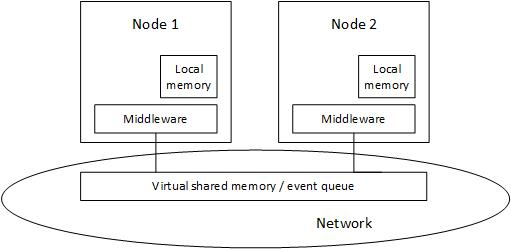
\includegraphics[width=0.8\textwidth,natwidth=610,natheight=642]{DistributedComputingSystemWith2nodes.jpg} 
	\captionsetup{format=plain,font=footnotesize,labelfont={bf,red},labelsep=quad,singlelinecheck=no}
	\caption[Distributed Computing System with 2 nodes]{
		\label{fig:distributedCoputingSystem} 
		\footnotesize{%
			A Distributed Computing System with 2 nodes.
		}
	}
\end{figure}

Figure \cref{fig:distributedCoputingSystem} illustrates the idea of a distributed computing system. Nodes 1 and 2 shares some virtual memory and/or event queue. The Middleware is a handles communication between the nodes and ensures the virtual memory is consistent throughout the network. The shared virtual memory is transparent to each node. 

Distributed systems offer many benefits over centralized systems including the following:
\begin{itemize}
	\item Scalability: It is easy to add notes to the system, should the size of the system increase.
	\item Redundancy: Several nodes can provide the same service, so if a node crashes, there are many to replace it. Additionally, from a cost perspective, each node does not have to be expensive, because many smaller nodes can be used as replacement.
\end{itemize}

\section{Thesis motivation}

\subsection{Siemens case}
Siemens Wind Power is among the leading windmill manufacturers in the world. 
Siemens builds wind farms of different sizes ranging form single mills to well above one hundred windmills \cite{simensOffShoreProjects, simensOnShoreProjects}.

In the current setup (see \cref{fig:currentSiemensSetup}) the Park Monitor is a central component and a SPOF (single point of failure).
The system is running on windows with a MSSQL database in the Park Monitor and MySQL on the windmills them self.
The windmills, Park Monitor and Park Regulator is connected with a gigabit network, witch currently has plenty of extra capacity.
The system handles more than 50 control points and 200 measurement points, and samples these every 50 ms.
The Park regulator is associated with the transformer station and regulated the power production when needed.
This component currently has a less than optimal work flow see \cref{fig:dataComputationSequence}.

Siemens has a need for their system to scale better and provide increased redundancy to avoid these SPOF's.
Siemens has a vision of removing the Park Monitor component and make it into a distributed system, distributed among the windmills (see \cref{fig:futureSiemensSetup}).
Also Siemens would like to look for ways to optimise the calculations done by the Park Regulator, 

\begin{figure}
	\centering
	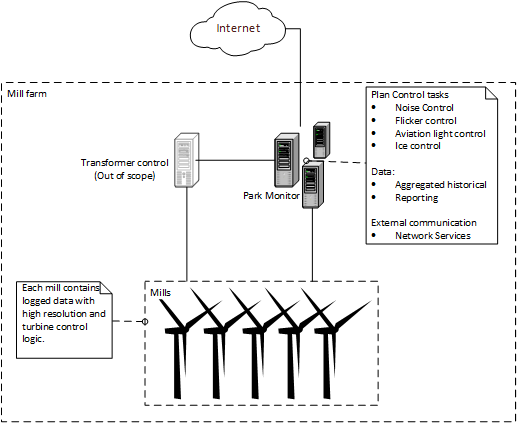
\includegraphics[width=0.7\textwidth,natwidth=610,natheight=642]{SystemOverviews.png} 
	\captionsetup{format=plain,font=footnotesize,labelfont={bf,red},labelsep=quad,singlelinecheck=no}
	\caption[Illustrates the current Siemens windmill farm setup]{
		\label{fig:currentSiemensSetup} 
		\footnotesize{%
			This figure illustrates the current Siemens windmill farm setup.
		}
	}
\end{figure}

\begin{figure}
	\centering
	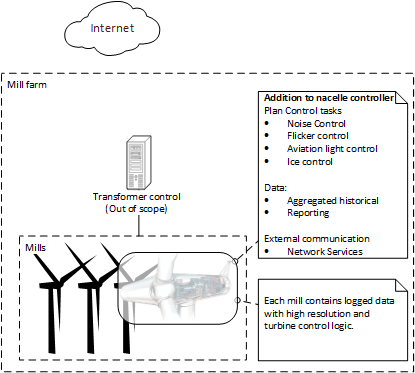
\includegraphics[width=0.7\textwidth,natwidth=610,natheight=642]{SystemOverviewsFuture.png} 
	\captionsetup{format=plain,font=footnotesize,labelfont={bf,red},labelsep=quad,singlelinecheck=no}
	\caption[Illustrates the future Siemens windmill farm setup]{
		\label{fig:futureSiemensSetup} 
		\footnotesize{%
			This figure illustrates the future Siemens windmill farm setup.
		}
	}
\end{figure}

\begin{figure}
	\centering
	\begin{sequencediagram} %Created using pgf-umlsd
		\newthread{reg}{:Park Regulartor}
		\newinst[2]{mill}{:Mill}
	
		\begin{sdblock}{each mill}{}
			\mess[1]{reg}{getCurrentStatus}{mill}
			\mess[1]{mill}{status}{reg}	
		\end{sdblock}
		
		\begin{call}{reg}{calculateAllSetpoints()}{reg}{}
		\end{call}
	
		\begin{sdblock}{each mill}{}
			\mess[1]{reg}{setNewSetpoint}{mill}
		\end{sdblock}
					
	\end{sequencediagram}

	\captionsetup{format=plain,font=footnotesize,labelfont={bf,red},labelsep=quad,singlelinecheck=no}
	\caption[Regulator calculation sequence]{
		\label{fig:dataComputationSequence} 
		\footnotesize{%
			Regulator calculation sequence.
		}
	}
\end{figure}
















\subsection{et eller andet}

Today windmills in windmill farm at Siemens are equipped with a computer for regulation, data and communication purposes. Every windmill are connected to a single server that aggregates data, perform calculations, store data and handle communication with the outside world. At Siemens up to 8 of theses servers are present pr. windmill farm and they pose the following problems:
\begin{itemize} 
	\item Single point of failure. Should a server fail, a part of the windmill farm will become unavailable.
	\item Low scalability. The servers does not scale with the number of windmills.
	\item Up performance of park regulator.
\end{itemize}

Therefor Siemens wishes to remove the servers by making every windmill farm a Distributed Computing System, utilizing free capacity of the computers already residing in every windmill. This would up the redundancy and scalability and the remove possibility of a single point of failure. A windmill farm must serve as single server which means ease of access must be maintained even though computation and data is distributed. This means routing traffic to a windmill with free capacity through a single interface, without external systems being aware of it.

% Today windmills in windmill farm are connected to a single server that aggregates data, perform calculations, store data and handle communication with the outside world. These servers do not scale well with the size of the windmill farm, and they are a single point of failure. Therefor Siemens wishes to remove the servers by utilizing free capacity of the computers already residing in every windmill. 
%Currently there is some limited redundancy in data and availability but this could be greatly improved by distributing data and communication to the windmills. 
%Ease of access must be maintained even though computation and data is distributed. 
%This means routing traffic to a windmill with free capacity through  a single interface.

\section{Thesis aim}

The purpose of this thesis is to design, implement and evaluate a framework and associated tools for distributed computing systems development. The case from Siemens Windpower is an example of a production environment where the framework could be utilized. The goal is not to make a framework that is specific to the Siemens case but to make a general framework for this and similar cases. 

This framework must be able to handle computation distributed on several nodes, communication between those nodes and distribution of data. 

The framework will be evaluated with regards to the existing Siemens solution using the following parameters: ... and will be done by comparing results obtained from a protocol 


%\begin{itemize}
%	\item How do we distribute a database and computation across a production environment in the best possible way?
%	\item How do we define and measure performance?
%	\item Can it provide data redundancy and outperform current systems?
%	\item How many windmills are needed before it makes sense to makes sense to distribute the server?
%\end{itemize}
%
%We aim to investigate the possibility of making a framework and associated tools for developing a distributed system. 
%This framework must be able to handle computation distributed on several nodes, communication between those nodes and distribution of data. 
%The communication can be built on top of existing standards as for instance DDS. Data distribution can be built using existing systems like MongoDB. 
%Distribution of computation tasks is the main research area and will be the focus of this thesis.
%
%In order to achieve distributed computation on several nodes the framework must be able to perform load balancing and control the distribution of tasks on the nodes in the system. 
%Furthermore the framework must have a single interface for control of, and interaction with, all the nodes.  
%The goal is to create a test system, that can distribute and perform tasks but also to be able to plan ahead of time and know if there is available computation time.
%
%The case from Siemens Windpower is an example of a production environment where the framework could be utilized. 
%Our goal is not to make a framework that is only  specific for this case but to make a general framework for this and similar cases.

\section{Approach}

\section{Outline}
The remainder of this thesis is organized into the following chapters...

\section{Audience}
This thesis is aimed at an audience with a basic knowledge of...

% include{dedication}
\chapter{Related work}
The popularity of wind energy has lead to massive research within the area. Generally the research is focused on a number of areas:

\begin{itemize}
	\item Optimization of turbine design and materials.
	\item Turbine and wind farm control.
	\item Integration of wind farms into existing power grids.
	\item Wind flow prediction and simulation.
	\item Wake flow optimization and simulation.
	\item Offshore wind farms.
\end{itemize}

%\section{Decentralized systems}
%With the coming era of Internet of Things (IoT) the focus on decentralized systems and autonomic agents is greater than ever.
%IoT devices must be able to communicate with each other directly without the need for an intermediate central server.
%Furthermore the IoT devices must be largely autonomous since they cannot rely on a lasting connection to a server for control.
%
%A new approach to control of wind farms is to utilize game theory\cite{AModelFreeApproachToWindFarmControl}.
%The turbines in a farm must cooperate to reach the desired goal of a chosen output.
%The game theory approach use an iterative learning algorithm that converges against the optimal output after n iterations.

\section{Aeolus}
The Aeolus project was a large scale EU supported project which lasted from may 2008 to april 2011. It included project partners from 
Aalborg University, Industrial Systems and Control Ltd in Glasgow, University of Zagreb, Energy Research Centre of the Netherlands and Vestas Wind Systems A/S.
The main objectives of the project was to research and develop predictions of flows and incorporate data from a network of sensors, as well as research and develop control paradigms that acknowledges the uncertainty in the modeling and dynamically manages the flow resource in order to optimize specific control objectives.
The project is relevant to this thesis because several approaches to control of a wind farm was evaluated.

One approach was the hierarchical approach which uses local control on the turbine level and global control on the wind farm level~\cite{HeirarchicalWindFarmControl}.
Setpoints for the global output of the wind farm are received by the controller on the wind farm level.
So is the output for each turbine and the maximum available output for each turbine.
The global controller calculates setpoints for each turbine based on the global setpoint and each turbines current and possible output.
The controllers on turbine level is responsible for reaching the setpoint calculated by the global controller as well as making each turbine reach the setpoint in the most optimal manner(gearing, avoid ice over, avoid oscillation).
The hierarchical approach is similar to the current approach used in the Siemens case.

Another approach was the decentralized feed-forward approach~\cite{DecentralisedFeedforwardControlOfWindFarms} which takes advantage of the fact that turbines are placed in a farm by letting upwind turbines feed wind data to downwind turbines. 
This allows downwind turbines to make adjustments to their production in order to exploit the coming wind in the best way.
Furthermore a restricted communication model is used allowing turbines only to communicate with their neighbors.
Using this decentralized feed-forward approach to control a wind farm can help even out the output of the farm since downwind turbines has additional information regarding wind speed to come to act upon. If upwind turbines power production is also a part of the feed-forward package downwind turbines may also be able to regulate overall wind farm production by evening out spikes from upwind turbines.
In addition by only communicating with neighboring turbines in order to achieve improvements in output the need for a centralized node is alleviated.

\section{Other related works}
The European Union has a number of sponsored projects beside the Aeolus project:
\begin{itemize}
	\item IRPWIND which aim to accelerate the transition towards low-carbon energy through better integration of the European research activities~\cite{IRPWIND}. The program has six subprogrammes:
	\begin{enumerate}
		\item Wind conditions
		\item Aerodynamics
		\item Structures and Materials
		\item Wind Integration
		\item Offshore Wind Energy
		\item Research Infrastructure
	\end{enumerate}
	\item INNWIND which focus is on accelerating the process of realizing the 20MW turbine~\cite{INNWIND}.
	\item EERA-DTOC which focus is on creating a software tool for optimizing offshore wind farm design and clusters of wind farms~\cite{eera-dtoc}.
\end{itemize}

Likewise the  United States of America has a number of projects most of them performed by Sandia National Laboratories or National Renewable Energy Laboratory:
\begin{itemize}
	\item SWiFT which focus is on wake effects, turbine control and rotor development~\cite{SWiFT}.
	\item Offshore Wind which focus on large rotor development and simulation algorithms~\cite{offshoreWind}.
	\item Active Power Control focus on using wind turbines for active control of the power grid~\cite{activePowerControl}.
\end{itemize}

The area of the supporting software architecture and software stack is not a topic that has received much attention, presumably because the prevailing solutions are proprietary and therefore not available for public research.
This thesis adds insight into which software components and technologies could be used in a wind farm thus filling in some of the gap in the research area.

%\subsection{Game theory control}
%A new approach to control of wind farms is to utilize game theory\cite{AModelFreeApproachToWindFarmControl}.
%The turbines in a farm must cooperate to reach the desired goal of a chosen output current.
%The game theory approach use an iterative learning algorithm that converges against the optimal output after n iterations.
%According to the above referenced article improvements on up to 25\% is possible compared to other algorithms currently in use.
\chapter{Analysis}
%% !TeX spellcheck = en_US
\chapter{Technologies}

\section{IP protocol Addressing methodologies}

The IP protocol defines 5 different communication methodologies\cite{MISSING REF}:
\begin{inparaenum}[{}]
	\renewcommand{\labelsep}{,,,dsf}	
	\item Broadcast
	\item Multicast
	\item Unicast
	\item Anycast
				
\end{inparaenum}

\subsection{Broadcast}
\subsection{Multicast}
\subsection{Unicast}

\section{Data Distribution Service}

\subsection{Node discovery}

\subsection{Real Time Streaming protocol}
\chapter{The Proposed Centralized Solution}\label{cha:existingSystem}

The \ref{PS:Q:Scalability} problem in the problem statement(\cref{sec:problemStatement}) requires a comparison between the decentralized solution and the current system at Siemens on different parameters. Ideally, for us to compare the two systems on equal terms, both systems should be implemented in the same environment. However, since we do not have access to the environment where the current system at Siemens is implemented, we have chosen to build our own version of the current Siemens system, in the same environment as the decentralized solution.

This version of the current Siemens system, from now on referred to as the centralized solution, is built from what Siemens has informed about the current Siemens system. The goal of the centralized solution is to create a foundation for a comparison between the decentralized solution and the current Siemens system, by making the system architecture around the regulation algorithm the only parameter changed from the centralized solution to the decentralized solution, thus ruling out the environment difference of the two systems as a parameter. This means the centralized solution is built to enable the collection of data that can be used to compare the two systems. As a result, we aim to compare the decentralized solutions test results with the centralized solutions test results, collected within the same environment, to more accurately address the \cref{PS:Q:Scalability} problem.

However in order to completely answer the \ref{PS:Q:Scalability} question, and compare the decentralized solution with the current Siemens system, another comparison must be introduced: A comparison between our centralized solution and the current Siemens system. This comparison is relevant in order to close the remaining 'comparison-gap' between the decentralized solution and the current Siemens system. This comparison will be a theoretical comparison between the centralized solution and the current Siemens system, and based on assumptions made when building the centralized solution.

As presented in \cref{fig:projectDiffOverview} there exist a difference between the current Siemens system and the centralized solution as well as a difference between the centralized solution and the decentralized solution, illustrated by deltas.

\begin{figure}[!h]
	\centering
	\begin{tikzpicture}[
	node distance = 0.3cm,
	auto,
	block/.style={draw, rectangle, text width=5em, text centered, minimum height=5cm}		
	]
% Place nodes
\node [block]			(Siemens)												[label=above:Siemens system]	{};
\node []					(SimCen)		[right = of Siemens] 	{$\Delta$};
\node [block]			(OurCent)		[right = of SimCen] 	[label=above:Centralized solution]	{};

\begin{scope}[on background layer]
\node [block] 		(Central) 	[fit=(Siemens) (OurCent), inner sep=20pt] {};
\node []					(CenDece)		[right = of Central] 	{$\Delta$};
\node [block]			(DeCent)		[right = of CenDece] 	[label=above:Decentralized solution] {};
\end{scope}

\end{tikzpicture}
	\captionsetup{format=plain,font=footnotesize,labelfont={bf,defaultCapFont},labelsep=quad,singlelinecheck=no}
	\caption[Comparison overview]{
		\label{fig:projectDiffOverview} 
		\footnotesize{%
			Comparison overview.
		}
	}
\end{figure}

The delta between the current Siemens system and the centralized solution is minimized as much as possible based on information about the current Siemens system delivered by Siemens Wind Power. Since the operation and regulation of the current Siemens system is proprietary the full system information is not available. To make up for the missing information a number of assumptions has been done about the current Siemens system which is also a part of the delta.
The delta between the centralized solution and decentralized solution describes the difference in operation of a centralized system and a decentralized system.

The thesis motivation (\cref{sec:ThesisMotivation}) describes a brief overview of the current system at Siemens. This chapter gives a detailed description of the key component of the current Siemens system: The regulation algorithm. Furthermore the chapter describes the centralized solution followed by a theoretical comparison between the centralized solution and the current Siemens system. 

\section{Regulation algorithm}\label{sec:cenRegAlgorithm}

The regulation algorithm is a key component of the current Siemens system and it is where new setpoints are calculated. Since the purpose of this thesis is not to improve any regulation algorithms, the regulation algorithm has been considered a black box in development of both the centralized and the decentralized solution. What is important to this thesis is that the algorithm used is the same in both the centralized and the decentralized solution, to make sure the two solutions are compared on the same terms. 

%To get as realistic a picture of the system as possible of the regulation algorithm, we tried to gain access to the algorithm Siemens currently use, but due to the regulation algorithm at Siemens being a commercial secret, this was not possible.

\begin{figure}
	\centering
	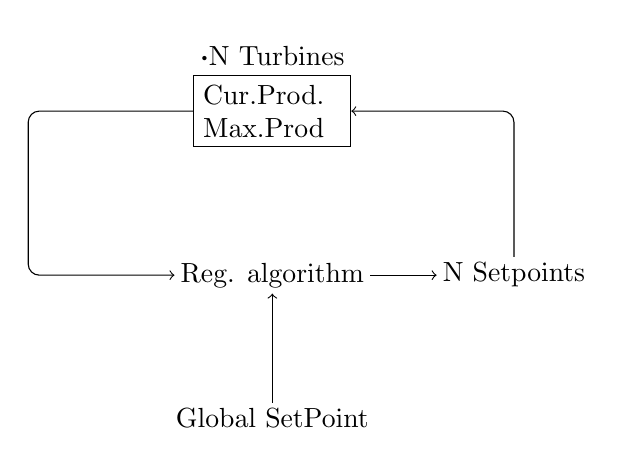
\begin{tikzpicture}[
	point/.style={inner sep=0pt}, %circle,minimum size=2pt,fill=red},
	textNode/.style={inner sep=2pt},
	hv path/.style={to path={-| (\tikztotarget)}},
	vh path/.style={to path={|- (\tikztotarget)}},
	skip loop h/.style={to path={-- ++(0,#1) -| (\tikztotarget)}},
	skip loop v/.style={to path={-- ++(#1,0) |- (\tikztotarget)}},
	graphs/every graph/.style={edges=rounded corners}
	]
	
% Place nodes
\matrix[row sep=1.4cm,column sep=.4cm] {
	\node [point]  		(p1x1)	{}; &&
	\node [rectangle]	(Turbine)		[draw, label=above:\textbf{$\cdot$}N Turbines, text width=50pt]	{Cur.Prod. Max.Prod}; &&
	\node [point]  		(p1x3)	{}; \\
	
	\node [point]  		(p2x1)			{}; &&
	\node [textNode]	(HPPP)		 	{Reg. algorithm}; &&
	\node [textNode]	(Setpoint)	{N Setpoints}; \\

	&& \node [textNode]  (gSetpoint)							{Global SetPoint}; \\
};
	
\graph[use existing nodes]{
	Turbine ->[skip loop v=-3.1cm] HPPP -> Setpoint ->[vh path] Turbine;
	gSetpoint -> HPPP;
};

\end{tikzpicture}



%\begin{tikzpicture}[
%	point/.style={inner sep=0pt}, %circle,minimum size=2pt,fill=red},
%	textNode/.style={inner sep=2pt},
%	hv path/.style={to path={-| (\tikztotarget)}},
%	vh path/.style={to path={|- (\tikztotarget)}},
%	skip loop h/.style={to path={-- ++(0,#1) -| (\tikztotarget)}},
%	skip loop v/.style={to path={-- ++(#1,0) |- (\tikztotarget)}},
%	graphs/every graph/.style={edges=rounded corners}
%	]
%	
%% Place nodes
%\matrix[row sep=1.5cm,column sep=.5cm] {
%	\node [point]  		(p1x1)	{}; &&
%	\node [rectangle]	(Turbine)		[draw, label=above:\textbf{$\cdot$}N Turbines, text width=50pt]	{Cur.Prod. Max.Prod}; &&
%	\node [point]  		(p1x3)	{}; \\
%	
%	\node [point]  		(p2x1)			{}; &&
%	\node [textNode]	(HPPP)		 	{HPPP}; &&
%	\node [textNode]	(Setpoint)	{\textbf{$\cdot$}N Setpoints}; \\
%
%	\node [textNode]  (gSetpoint)										{Global SetPoint}; &&
%	\node [rectangle]	(Data)			[draw, text width=50pt] {Cur.prod  Max.Prod};\\
%};
%
%\node [textNode,right of=Data] {~~~~~~~~~~~~~~~~~\textbf{$\cdot$}N Turbines};
%	
%\graph[use existing nodes]{
%	Turbine ->[skip loop v=-2.7cm] HPPP -> Setpoint ->[vh path] Turbine;
%	gSetpoint.east -> HPPP;
%	Data -> HPPP;
%};
%
%\end{tikzpicture}

	\captionsetup{format=plain,font=footnotesize,labelfont={bf,defaultCapFont},labelsep=quad,singlelinecheck=no}
	\caption[Centralized input/output parameters of the regulation algorithm]{
		\label{fig:ioCenRegAlg} 
		\footnotesize{%
			Centralized input/output parameters of the regulation algorithm.
		}
	}
\end{figure}

With the algorithm being a black box, the input/output parameters of the regulation algorithm was studied to provide the correct communication circumstances for the regulation algorithm. \Cref{fig:ioCenRegAlg} presents a simple input/output overview of the regulation algorithm. Input/output parameters of the regulation algorithm are as follows:

\begin{description}
	\item The \textbf{global setpoint} of the wind farm. This is the production goal of the wind farm. %Which means all turbines combined should produce.
	\item The \textbf{setpoint} of each turbine, calculated from the regulation algorithm. 
	\item The \textbf{current production} of the turbine.
	\item The \textbf{maximum production} of the turbine. In real-life, this parameter is amongst others determined from the wind conditions around the turbine.
\end{description}

These input/output parameters of the regulation algorithm is simplified compared to the current Siemens system. The data used is more og less irrelevant for the purpose of this thesis as long as both the decentralized solution and the centralized solution are using the same data and as long as both systems are able to perform the same simple regulation.

\section{Regulation cycle}\label{sec:currentSystemCen} 

The first area studied when building the centralized solution, was building the frames for the regulation algorithm (see \cref{sec:cenRegAlgorithm}), meaning how to communicate the input/output around the centralized solution.

This section describes the components of a regulation cycle in the centralized solution. The regulation cycle consist of a number of steps presented in \cref{fig:timingCentral}.

\begin{figure}[!h]
	%The figure show how regulation time differs central vs decantral
	

{ %The brackets issolate the enviroment

\tikzstyle{line}		 	= [draw]

\makeatletter
\ifcsname c@wavenum\endcsname %Only create one counter
\else
	\newcounter{wavenum}
\fi
\makeatother

\newcommand*{\bitvector}[3]{
  \draw[fill=#3] (t_cur) -- ++( .1, .3) -- ++(#2-.2,0) -- ++(.1, -.3)
                         -- ++(-.1,-.3) -- ++(.2-#2,0) -- cycle;
  \path (t_cur) -- node[anchor=mid](textNode) {#1} ++(#2,0) node[time] (t_cur) {};
  }

% \known{val}{length}
\newcommand*{\known}[2]{
    \bitvector{#1}{#2}{white}
}

% \unknown{length}
\newcommand*{\unknown}[2]{
    \bitvector{#1}{#2}{black!20}
}

% \nextwave{name}
\newcommand{\nextwave}[1]{
  %\path (0,\value{wavenum}) node[time] (t_cur) {};
   \path (0,\value{wavenum}) node[left] {#1} node[time] (t_cur) {};
  \addtocounter{wavenum}{-1}
}

\newcommand{\timeSpanLabel}{
	\node (CycleTimeLabel) [rectangle, above = 0.7cm of textNode, inner sep=0pt] {Regulation cycle time};	  
}

\newcommand{\timeSpanA}{
	\node (t_timeSpanA) [point, above = 0 of t_cur] {};	  
}

\newcommand{\timeSpanB}{
	\node (t_timeSpanB) [point, above =0 of t_cur] {};

  \graph[use existing nodes]{
  	t_timeSpanA --[time span=1cm] CycleTimeLabel;
   	CycleTimeLabel.south --[time span=-0.24cm] t_timeSpanB;
  }; 
    	
}


%%% End of timing.sty
\begin{tikzpicture}[
	point/.style={inner sep=0pt}, %circle,minimum size=2pt,fill=red},
	draw=black, 
	yscale=.8,
	xscale=1,
	hv path/.style={to path={-| (\tikztotarget)}},
	vh path/.style={to path={|- (\tikztotarget)}},
	skip loop v/.style={to path={-- ++(#1,0) |- (\tikztotarget)}},		
	skip loop h/.style={to path={-- ++(0,#1) -| (\tikztotarget)}},
	time span/.style={to path={-- ++(0,#1) -| (\tikztotarget)}},
	graphs/every graph/.style={edges=rounded corners}	
	]
	
  \tikzstyle{time}=[coordinate]
  \setlength{\unitlength}{1cm}
  \setcounter{wavenum}{0}
    
  %\nextwave{Regulation Time} \unknown{SendData}{2} \known{WaitForData}{5} \unknown{ReciveData}{2} \unknown{Calculate}{2}\unknown{SendSP}{2}
  \nextwave{Park Pilot} \unknown{reqStates}{1.8} \known{wait}{2} \unknown{readStates}{2} \unknown{regAlg.}{1.7} \unknown{sendSetpoints}{2.6}
  
  \nextwave{Turbine} \known{wait}{1.8} \unknown{replyState}{2} \known{wait}{6.3} \unknown{receiveSetpoint}{2.9}
    
  
\end{tikzpicture}
}

	\caption{The regulation cycle of the centralized solution}
	\label{fig:timingCentral}
\end{figure}

\subsection{Get turbine states}\label{sec:getTurbineStates}

In order for the Park Pilot to calculate turbine setpoints, the Park Pilot must have the state of all turbines.

\begin{figure}
	\centering
	\begin{sequencediagram} %Created using pgf-umlsd
		\newthread{parkPilot}{:Park Pilot}
		\newthread{turbineDataReplier}{:Turbine Data Replier}
		\newinst{turbine}{:Turbine}
	
		\begin{sdblock}{each turbine}{}
			\mess[1]{parkPilot}{reqState}{turbineDataReplier}
			\begin {call}{turbineDataReplier}{readState()}{turbine}{return state}
			\end {call}
			\mess[1]{turbineDataReplier}{replyState}{parkPilot}
		\end{sdblock}				
	\end{sequencediagram}

	\captionsetup{format=plain,font=footnotesize,labelfont={bf,defaultCapFont},labelsep=quad,singlelinecheck=no}
	\caption[First part of the regulation cycle]{
		\label{fig:getStatesOfTurbines} 
		\footnotesize{%
			First part of the regulation cycle: Getting the state of all turbines.
		}
	}
\end{figure}

A simple overview of the first part of the regulation cycle is presented on \cref{fig:getStatesOfTurbines}. This part of the regulation cycle is implemented using the RTI Connext Request-Reply implementation~\cite{rtiConnextUsersManual}. The three primary objects of this part of the regulation cycle are:

\begin{description}
	\item [Park Pilot] The Park Pilot requests the current state of all turbines and calculates setpoints when states has been received.
	\item [Turbine Data Replier] The replier object handles the request and sends a reply.
	\item [Turbine] The underlying turbine object is the interface to the Turbine, which handles communication with the underlying database with simulation data.
\end{description}

The Park Pilot sends a request to a specific DDS Topic and then waits until it has received a reply from all the turbines subscribing to this DDS Topic, which in our case is all turbines. In a real-life implementation of the centralized solution, a timer should be implemented to determine how long to wait for the replies, and maybe even mark a turbine as offline, if a given turbine does not reply within that time frame. However, since this is a prototype for comparison purposes, this functionality has not been implemented. The request message, sent from the Park Pilot, contains the regulation cycle time, which is only used for data logging purposes (i.e. not used by the turbines).

The Turbine Data Replier is instantiated with the Turbine object and runs on every turbine. After instantiation, the Turbine Data Replier goes into an infinite loop which first waits infinitely until a request is received, reads turbine data from the Turbine object and finally sends a reply containing the data to the Park Pilot. Ideally, the Turbine Data Replier object should have been implemented as a listener on the request topic using RTI Connext SimpleReplier~\cite{rtiConnextUsersManual}. However, we could not get it to work using the SimpleReplier but waiting infinitely for a request works just as well for our purpose.

The Turbine object is the interface to the actual Turbine. The primary functionality of this object is to change state when a new setpoint is assigned to the object. Furthermore it reads data from the underlying MongoDB database. 

\subsection{Calculate setpoints (regAlgorithm)}\label{sec:calculateSetpoints}

When the Park Pilot has received the states of all turbines the setpoints for all turbines are calculated. Since we don't have access to Siemens' regulation algorithm (see \cref{sec:cenRegAlgorithm} for explanation), we have developed our own simple regulation algorithm. The code for this regulation algorithm is presented on \cref{fig:cenRegAlgCode}.

\begin{figure}[!h]
	\centering
%	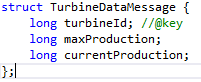
\includegraphics[width=0.3\textwidth,natwidth=250,natheight=200]{turbineDataMessage.PNG} 
	\begin{lstlisting}[language=C++,tabsize=2,basicstyle=\small]
void CentralizedParkPilot::regAlgorithm(
	uint_fast32_t globalSetpoint,
	LoanedSamples<TurbineDataMessage> &turbines)
{
	int availableTurbinesCount = turbines.length();

	typedef LoanedSamples<TurbineDataMessage>::iterator iterator;
	long localSetpoint = 0;

	for (iterator it = turbines.begin(); it != turbines.end(); ++it) {
		if (it->info().valid_data) {

			if (it->data().currentProduction >= it->data().maxProduction) {
				availableTurbinesCount--;
			}
		}
		else
			availableTurbinesCount--;
	}

	for (iterator it = turbines.begin(); it != turbines.end(); ++it) {
		if (it->info().valid_data) {
			if (availableTurbinesCount <= 0)
				localSetpoint = globalSetpoint;
			else
				localSetpoint = globalSetpoint / availableTurbinesCount;

			if (localSetpoint > it->data().maxProduction) {
				localSetpoint = it->data().maxProduction;
			}

			_turbineOutlets[it->data().turbineId - START_ID]->
						setSetpoint(localSetpoint);
					
			_turbineOutlets[it->data().turbineId - START_ID]->publishData();
		}
	}
}
	\end{lstlisting}
	\captionsetup{format=plain,font=footnotesize,labelfont={bf,defaultCapFont},labelsep=quad,singlelinecheck=no}
	\caption[The regulation algorithm of the centralized solution]{
		\label{fig:cenRegAlgCode} 
		\footnotesize{%
			Code for the centralized regulation algorithm used to calculate setpoints.
		}
	}
\end{figure}


Our regulation algorithm works by first determining how many turbines that are available for production. This is done going through every turbine, checking if they currently hit their maximum production capacity. If a given turbine is producing at maximum capacity, a greater load cannot be assigned to it and the available turbine count is reduced. 

Next the setpoint for every turbine is calculated using this simple formula: $setpoint=globalSetpoint/availableTurbines$. If this new setpoint is higher than the maximum capacity of a given turbine, the turbine is set to produce at maximum capacity. If this happens, a gap between the maximum capacity and the calculated setpoint is left unhandled, and the wind farm is under-producing until the next cycle, where a new set of setpoints are calculated, with one less available turbine. Hence this gap will eventually be closed unless the maximum capacity of the entire park is reached.

\subsection{Send setpoints}

\Cref{fig:sendSetpoints} presents a simple overview of the last part of the regulation cycle. This part of the regulation cycle is implemented using RTI Connext Publish-Subscribe implementation~\cite{rtiConnextUsersManual}. The primary objects are:

\begin{description}
	\item [Park Pilot] Explained in \cref{sec:getTurbineStates}.
	\item [Turbine Outlet] The Park Pilots implementation of a given turbine. One Turbine Outlet is instantiated on the Park Pilot for each turbine in the park. Writing data to each turbine is handled from this object.
	\item [Setpoint Listener] The listener object called when when a new setpoint is published. One Setpoint Listener are instantiated on each turbine.
	\item [Turbine] Explained in \cref{sec:getTurbineStates}.
\end{description}

After calculating the setpoints (\cref{sec:calculateSetpoints}), the Park Pilot sends a new setpoint to each turbine. The Park Pilot sets the setpoint of the Turbine Outlet before publishing the Data.

\begin{figure}[!h]
	\centering
	\begin{sequencediagram} %Created using pgf-umlsd
		\newthread{parkPilot}{:Park Pilot}
		\newinst{turbineOutlet}{:Turbine Outlet}
		\newinst{setPointListener}{:Setpoint Listener}
		\newinst{turbine}{:Turbine}
	
		\begin{sdblock}{each turbineOutlet}{}
			\begin {call}{parkPilot}{setSetpoint()}{turbineOutlet}{}
			\end {call}
			\begin {call}{parkPilot}{publishData()}{turbineOutlet}{}
				\mess[1]{turbineOutlet}{write}{setPointListener}
				\begin {call}{setPointListener}{setSetpoint()}{turbine}{}
				\end {call}
			\end {call}
		\end{sdblock}				
	\end{sequencediagram}

	\captionsetup{format=plain,font=footnotesize,labelfont={bf,defaultCapFont},labelsep=quad,singlelinecheck=no}
	\caption[Last part of the regulation cycle]{
		\label{fig:sendSetpoints} 
		\footnotesize{%
			Last part of the regulation sequence: Sending setpoints to all turbines.
		}
	}
\end{figure}

The main purpose of Turbine Outlet object is to register and publish setpoints to each turbine. Upon instantiation, the Turbine Outlet registers the turbine id as a RTI Connext key~\cite{rtiConnextUsersManual} to the setpoint topic and saves the handle object. Saving the handle upon registration and using the handle when writing improves performance~\cite{DDSInstanceHandlet}, which is why the handle is saved with the object. Lastly the object writes the data to the topic.

The Setpoint Listener object is a listener on the setpoint topic. The setpoint topic is configured with as a Content Filtered Topic~\cite{rtiConnextUsersManual}, so the listener only reacts to messages with a key that equals the turbines id (see \cref{sec:ddsConfigCen} for DDS configuration). When Setpoint Listener object is invoked, the new setpoint is saved to the Turbine object, which updates the state of the turbine.

\section{DDS configuration}\label{sec:ddsConfigCen} 

The key component used for communication is DDS (see \cref{sec:DSM}). This section describes how DDS has been configured for the centralized solution.

\subsection{Interface Description Language}\label{sec:cenIdl}

The data transfer objects (DTO) used when sending messages from the turbines to the Park Pilot, and the other way around, is created using the RTI Connext Interface Description Language~\cite{rtiConnextUsersManual}. DTOs are defined in an IDL file (see \cref{fig:cenTurbineDataMessage} for IDL example). From there the actual implementations of the IDL definitions are auto generated from the command prompt using the \textit{rtiddsgen}~\cite{rtiConnextUsersManual} command.

\begin{figure}[!h]
	\centering
%	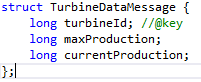
\includegraphics[width=0.3\textwidth,natwidth=250,natheight=200]{turbineDataMessage.PNG} 
	\begin{lstlisting}[language=C++,tabsize=2,basicstyle=\small]
	struct TurbineDataMessage {
		long turbineId; //@key
		long maxProduction;
		long currentProduction;	
	}	
	\end{lstlisting}
	\captionsetup{format=plain,font=footnotesize,labelfont={bf,defaultCapFont},labelsep=quad,singlelinecheck=no}
	\caption[Centralized turbine reply message]{
		\label{fig:cenTurbineDataMessage} 
		\footnotesize{%
			The the reply message .idl file sent from the turbines to the Park Pilot in the centralized solution.
		}
	}
\end{figure}

The IDL definitions are defined from looking at what data to transfer between the turbines and the Park Pilot. \Cref{fig:cenTurbineDataMessage} is for example the IDL definition of the data transfer object used as reply from the turbines to the Park Pilot.

%\subsection{Topics}
%
%Including the topics generated from the RTI Connext Request-Reply implementation~\cite{rtiConnextUsersManual} the following topics are used:
%
%\begin{figure}
%	\centering
%	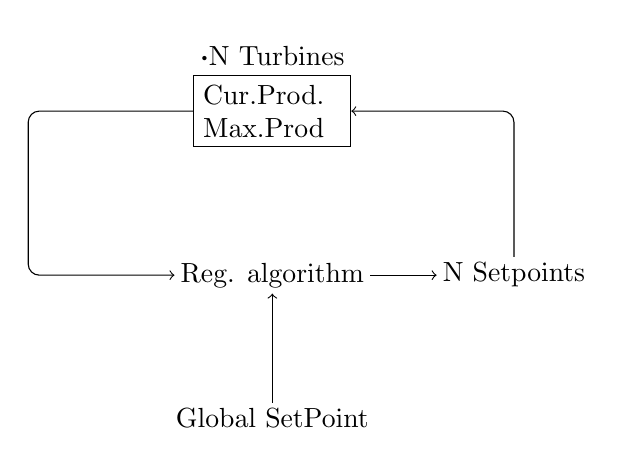
\begin{tikzpicture}[
	point/.style={inner sep=0pt}, %circle,minimum size=2pt,fill=red},
	textNode/.style={inner sep=2pt},
	hv path/.style={to path={-| (\tikztotarget)}},
	vh path/.style={to path={|- (\tikztotarget)}},
	skip loop h/.style={to path={-- ++(0,#1) -| (\tikztotarget)}},
	skip loop v/.style={to path={-- ++(#1,0) |- (\tikztotarget)}},
	graphs/every graph/.style={edges=rounded corners}
	]
	
% Place nodes
\matrix[row sep=1.4cm,column sep=.4cm] {
	\node [point]  		(p1x1)	{}; &&
	\node [rectangle]	(Turbine)		[draw, label=above:\textbf{$\cdot$}N Turbines, text width=50pt]	{Cur.Prod. Max.Prod}; &&
	\node [point]  		(p1x3)	{}; \\
	
	\node [point]  		(p2x1)			{}; &&
	\node [textNode]	(HPPP)		 	{Reg. algorithm}; &&
	\node [textNode]	(Setpoint)	{N Setpoints}; \\

	&& \node [textNode]  (gSetpoint)							{Global SetPoint}; \\
};
	
\graph[use existing nodes]{
	Turbine ->[skip loop v=-3.1cm] HPPP -> Setpoint ->[vh path] Turbine;
	gSetpoint -> HPPP;
};

\end{tikzpicture}



%\begin{tikzpicture}[
%	point/.style={inner sep=0pt}, %circle,minimum size=2pt,fill=red},
%	textNode/.style={inner sep=2pt},
%	hv path/.style={to path={-| (\tikztotarget)}},
%	vh path/.style={to path={|- (\tikztotarget)}},
%	skip loop h/.style={to path={-- ++(0,#1) -| (\tikztotarget)}},
%	skip loop v/.style={to path={-- ++(#1,0) |- (\tikztotarget)}},
%	graphs/every graph/.style={edges=rounded corners}
%	]
%	
%% Place nodes
%\matrix[row sep=1.5cm,column sep=.5cm] {
%	\node [point]  		(p1x1)	{}; &&
%	\node [rectangle]	(Turbine)		[draw, label=above:\textbf{$\cdot$}N Turbines, text width=50pt]	{Cur.Prod. Max.Prod}; &&
%	\node [point]  		(p1x3)	{}; \\
%	
%	\node [point]  		(p2x1)			{}; &&
%	\node [textNode]	(HPPP)		 	{HPPP}; &&
%	\node [textNode]	(Setpoint)	{\textbf{$\cdot$}N Setpoints}; \\
%
%	\node [textNode]  (gSetpoint)										{Global SetPoint}; &&
%	\node [rectangle]	(Data)			[draw, text width=50pt] {Cur.prod  Max.Prod};\\
%};
%
%\node [textNode,right of=Data] {~~~~~~~~~~~~~~~~~\textbf{$\cdot$}N Turbines};
%	
%\graph[use existing nodes]{
%	Turbine ->[skip loop v=-2.7cm] HPPP -> Setpoint ->[vh path] Turbine;
%	gSetpoint.east -> HPPP;
%	Data -> HPPP;
%};
%
%\end{tikzpicture}
%
%	\captionsetup{format=plain,font=footnotesize,labelfont={bf,defaultCapFont},labelsep=quad,singlelinecheck=no}
%	\caption[Regulation aslgorithm input/output parameters]{
%		\label{fig:ioRegAlg} 
%		\footnotesize{%
%			Input/output parameters of the regulation algorithm.
%		}
%	}
%\end{figure}

\subsection{Choosing quality of service parameters}\label{sec:choosingQosParams}

Quality of Service (QoS) parameters are parameters used to determine the behavior of a system using RTI Connext DDS. As such, setting the right QoS parameters for the centralized solution is important in order to duplicate the behavior of the current system at Siemens as close as possible. 

In order to decide the QoS parameters for the centralized solution, the QoS XML file from the current system at Siemens was provided by Siemens (see \cref{appendix:siemensQosFile} for the QoS XML file). Thus QoS parameters for the centralized solution has been set using this file, which presents many different QoS profiles.

The Siemens QoS XML file specifies one \textit{DomainParticipantFactory} profile. This profile has been applied to the solution and parameters irrelevant to the purpose of this thesis has been removed from the profile. 

The Siemens QoS XML file specifies two \textit{DomainParticipant} profiles. One using UDPv4 and one using DTLS as transport plugin. The one using UDPv4 has been chosen for the centralized solution, since DTLS encryption and decryption is an unnecessary overhead, that either should be introduced to both the centralized- and the decentralized solution or to neither, for the two solutions to be compared on the same terms. Thus for simplicity neither of the solutions introduce DTLS.

As for \textit{DataReaders}, \textit{DataWriters} and \textit{Topics}, the file specifies multiple profiles the use of which is unknown. Thus it is unknown which ones has been used for the part of the system that is implemented with the centralized solution. Furthermore since the centralized solution is a simplified version of the current Siemens system it will not need the number of \textit{DataReaders}, \textit{DataWriters} and \textit{Topics} that the current Siemens system apply.

Each Qos parameter in every QoS profile has been evaluated and the parameters relevant to the purpose of this theses has been applied to the centralized solution, based on assumptions about the current Siemens system. The QoS XML file roughly presents profiles that combines the following parameters in different ways:

\paragraph{Reliability} is the QoS parameter, which determines whether or not data published by a \textit{DataWriter} will be reliably delivered by the DDS framework to matching \textit{DataReaders}~\cite{rtiConnextUsersManual}. The three levels of reliability presented by the different profiles are:

\begin{itemize}
	\item \textbf{Best effort reliability} profiles are configured so data samples are sent once and missed samples are acceptable.
	\item \textbf{Reliable} profiles are configured to make sure that data sent is received and missed samples are resent. \textit{DataWriters} will send samples reliably to \textit{DataReaders}, buffering sent data until they have been acknowledged as being received by \textit{DataReaders} and resending any samples that may have been lost during transport. The \textit{DataWriter} buffer of this configuration is set to the size of one message, which means only the newest message is resent. This implies that an unacknowledged sample may be overwritten and thus lost. 
	\item \textbf{Strictly reliable} profiles are configured like reliable profiles, but with a larger \textit{DataWriter} buffer. Increasing the \textit{DataWriter} buffer size will decrease the chance of unacknowledged samples being overwritten. Thus \textit{DataReaders} are ensured all messages sent by the \textit{DataWriters}.
\end{itemize}

\paragraph{Durability} controls whether or not, and how, published samples are stored by the \textit{DataWriter} application for \textit{DataReaders} that are found after the samples were initially written, thus allowing new \textit{DataReaders} to receive data sent before they were created. The levels of durability presented by the different profiles are:

\begin{itemize}
	\item \textbf{No durability} profiles are configured not to store any samples for newly discovered \textit{DataReaders}.
	\item \textbf{Local durability} profiles are configured such that \textit{DataWriters} will store and send previously published samples for delivery to newly discovered \textit{DataReaders} as long as the \textit{DataWriter} still exists.
\end{itemize}

\paragraph{Throughput} is configured using the batch~\cite{rtiConnextUsersManual} parameter, which can be used to decrease the amount of communication overhead associated with the transmission and (in case of reliable communication) acknowledgment of small samples at the expense of latency. This is done by batching many smaller samples to be sent in a single large packet, which increases network utilization and thus throughput in terms of samples per second. The two levels of throughput presented by the different profiles are:

\begin{itemize}
	\item \textbf{Regular throughout} profiles are configured to avoid batching of samples, thus data samples and (in case of reliable communication) acknowledgment message are sent individually.
	\item \textbf{High throughput} profiles are configured such that \textit{DataWriters} will batch data in order to increase throughput.
\end{itemize}

The many profiles in the Siemens QoS XML file (\cref{appendix:siemensQosFile}) are presumably made for many different purposes. For building the centralized solution, the profile using \textbf{Strictly reliable}, \textbf{No durability} and \textbf{Regular throughput} configurations was chosen based on the following assumptions about the current Siemens system:

\begin{itemize}
	\item \textbf{Strictly reliable} messaging is important for the Park Pilot to compute setpoints for each turbine, since states of all turbines are needed in order to calculate setpoints. Thus resending a sample data if the sample data is dropped is needed in order to calculate setpoints. 
	\item \textbf{No durability} is needed for the regulation algorithm. If a new turbine is discovered, the turbine have no need of receiving old requests or setpoints. The turbine only needs to make itself available to requests from the Park Pilot and thereby be taken into account, which is done automatically by \textit{Connext} when a the new \textit{DataReader} of the turbine is discovered.  
	\item \textbf{Regular throughput} provides the best performance for the regulation cycle. Batching data samples does not make any sense for the centralized solution since during the regulation cycle, a given node can only fall one message behind and since heartbeats and data samples are batched per default.
\end{itemize}

The chosen profile from the current Siemens system QoS XML, from which QoS profiles for the centralized solution has been built, is the profile called \textit{SwpStrictReliableNoDurability} (\cref{appendix:siemensQosFile}).


\subsection{Detailed quality of service evaluation} \label{sec:detailedQoSDesc}

The section provides a detailed evaluation of every parameter of the chosen profiles of the centralized solution QoS XML file, including the QoS parameters deemed irrelevant and thereby removed from the QoS file provided by Siemens (\cref{appendix:siemensQosFile}). See \cref{appendix:centralizedQosFile} for centralized solution QoS XML file. Removed parameters are marked with '(removed)' and commented out in the figures.

\paragraph{Participant factory} (\cref{fig:parFacQos}) QoS parameters has been evaluated as follows:

\begin{itemize}
	\item \textbf{autoenable\_created\_entities (removed)} determines whether or not participants should be enabled upon initialization. For the centralized solution the default value (enabled) for this parameter is sufficient.
	\item \textbf{logging} is set for all participants and occurs on both errors and warning messages concerning the underlying platform (hardware or OS) on which \textit{RTI Connext} is running. A warning indicates that \textit{RTI Connext} is taking an action that may not be what was originally intended. This parameter is set since the current Siemens system uses this setting and for debugging purposes.
\end{itemize}

\begin{figure}
\begin{lstlisting}[language=XML]
<participant_factory_qos>
	<!--entity_factory>
		<autoenable_created_entities>false</autoenable_created_entities>
	</entity_factory-->
	<logging>
		<verbosity>WARNING</verbosity>
		<category>PLATFORM</category>
		<print_format>VERBOSE_TIMESTAMPED</print_format>
		<output_file>ddsadaptor.log</output_file>
	</logging>
</participant_factory_qos>
\end{lstlisting}
\caption[Participant factory QoS parameters]{
		\label{fig:parFacQos} 
		\footnotesize{Participant factory QoS parameters.}
	}
\end{figure}

\paragraph{Participant} (\cref{fig:parQos}) QoS parameters has been evaluated as follows:
 
\begin{itemize}
	\item \textbf{database} configures how \textit{RTI Connext} manages its internal database, which stores information about entities created locally as well as remote entities found during the discovery process. Database thread has been set to wake up and delete removed records 1 ns after a given domain participant is destroyed for cleanup purposes.
	
	\item \textbf{transport\_builtin} configures the built-in transport plugins (UDPv4/IP, UDPv6/IP, TCP/IP, TLS, DTLS, shared memory, etc.) used by the \textit{DomainParticipants}. By default UDPv4 and shared memory plugins are enabled. For the centralized solution, the shared memory plugin is disabled (set to UDPv4 only) such that applications running on the same node do not use shared memory to communicate. This is done since our test setup only involves 3 test machines, each simulating a number of turbines. As such, communication through shared memory is not acceptable, because the turbines must communicate as if they are separate machines.
	
	\item \textbf{receiver\_pool (removed)} configures the internal \textit{Connext} thread used to process the data received from a transport. As such, the \textbf{buffer\_size} configures the size of the receive buffer in bytes. The default value of this property is set to the largest message size of all installed transports, which is needed for the centralized solution. Thus the default value is sufficient and the custom value used in the current Siemens system is removed from the centralized solutions QoS file.
	
	\item \textbf{ignore\_nonup\_interfaces (removed)} property allows/disallows the use of interfaces that are not reported as UP (by the operating system) in the UDPv4 transport. Setting this value to 0 supports the communication scenarios in which interfaces are enabled after the participant is created. This parameter has been removed since the centralized solution do not have any interfaces that are enabled after the participant is created. Thus the centralized solution uses the default value of 1 which means interfaces that are reported as down is not supported.
	
	\item \textbf{multicast\_enabled (removed)} parameter is used to configure if the transport plugin (in this case UDPv4) should use multicast for sending and receiving. By removing this parameter the default value is used, which allows multicast on all network interfaces allowed for multicast that is found up and running when the plugin is instantiated. The centralized solution is \textbf{not} supposed to use multicast for sending and receiving data used in context of the regulation cycle, however multicast is acceptable for discovery of \textit{DomainParticipants}. Thus this parameter is set to default for discovery purposes.
	
	Note that we have not set any multicast addresses on the \textit{DataReader} QoS profile (see \textit{DataReader} QoS parameters later in this section), which means multicast is not used for sending and receiving data in the context of the regulation cycle.
	
	\item \textbf{message\_size\_max} configures the maximum size of a message in bytes. This value must be set before the transport plugin is registered, such that \textit{Connext} can properly use the plugin. For the purpose of the centralized solution this value is more or less irrelevant, since it's only a max value. The value of this parameter just have to be larger than the largest message size in bytes plus any overhead (ie. $message\_size\_max \geq largest\_msg + msg\_overhead$). The largest message of the centralized solution contains $3\cdot64bit=192bit$. Thus to maintain similarity to the current Siemens system and since any larger value has no influence on our test results, the value of this parameter is left as the value used by the current Siemens system at a size of 65535 bytes.
	
	\item \textbf{send\_socket\_buffer\_size} configures the size of the send buffer in bytes. This value must be greater than or equal to the value of the \textit{message\_size\_max} parameter. For the purpose of the centralized solution this value have to be big enough to contain enough messages to cover the \textit{DataWriter} history QoS (see DataWriter QoS history parameter later in this section), with regards to the largest centralized message size of $3\cdot64bit=192bits$ plus any message overhead. Thus a value of 65535 bytes is more than enough, and the value is kept to maintain similarity to the current Siemens system.
	
	\item \textbf{recv\_socket\_buffer\_size} configures the size of the receive buffer. This value must be greater than or equal to the value of the \textit{message\_size\_max} parameter. For the purpose of the centralized solution this value have to be big enough to contain enough messages to cover \textit{DataReader} history QoS (see DataReader QoS history parameter later in this section) with regards to the largest centralized message size of $3\cdot64bit=192bits$ plus any message overhead. 
\end{itemize}

\begin{figure}
\begin{lstlisting}[language=XML]
<participant_qos>
	<database>
		<shutdown_cleanup_period>
			<sec>DURATION_ZERO_SEC</sec>
			<nanosec>1</nanosec>
		</shutdown_cleanup_period>
	</database>
	<participant_name>
		<name>Siemens Wind Power DDS Adaptor</name>
	</participant_name>
	<transport_builtin>
		<mask>UDPv4</mask>
	</transport_builtin>
	<!--receiver_pool>
		<buffer_size>65535</buffer_size>
	</receiver_pool-->
	<property>
		<value>
			<!--element>
				<name>dds.transport.UDPv4.builtin.ignore_nonup_interfaces</name>
				<value>0</value>
			</element>
			<element>
				<name>dds.transport.UDPv4.builtin.multicast_enabled</name>
				<value>0</value>
			</element-->
			<element>
				<name>dds.transport.UDPv4.builtin.parent.message_size_max</name>
				<value>65535</value>
			</element>
			<element>
				<name>dds.transport.UDPv4.builtin.send_socket_buffer_size</name>
				<value>65535</value>
			</element>
			<element>
				<name>dds.transport.UDPv4.builtin.recv_socket_buffer_size</name>
				<value>2097152</value>
			</element>
		</value>
	</property>
</participant_qos>
\end{lstlisting}
\caption[Participant QoS parameters]{
		\label{fig:parQos} 
		\footnotesize{Participant QoS parameters.}
	}
\end{figure}

\FloatBarrier

\paragraph{Topic} QoS parameters are not presented by the Current Siemens System QoS XML file and thus no \textit{Topic} QoS profile has been applied to the centralized solution. 

\paragraph{DataWriter} QoS parameters has been set after the profile \textit{SwpStrictReliableNoDurability} from the current Siemens system QoS XML file (\cref{appendix:siemensQosFile}), as discussed in \cref{sec:choosingQosParams}. Combining the \textit{SwpStrictReliableNoDurability} profile with the two underlying base profiles (\textit{SwpReliableNoDurability} and \textit{SwpBestEffort}) we get the QoS parameters presented on \cref{fig:writerQoS}. The DataWriter parameters presented on \cref{fig:writerQoS} has been evaluated as follows:

\begin{itemize}
	\item \textbf{liveliness (removed)} configures how \textit{Connext} determines whether a \textit{DataWriter} is alive, meaning if the \textit{DataWriter} is reachable by other DDS entities. A \textit{lease\_duration} specifies the maximum time at which packets that indicate that the \textit{DataWriter} is still alive are sent to matching \textit{DataReaders}. If the \textit{lease\_duration} is exceeded, an \textit{on\_liveliness\_changed} event is triggered on subscribers within the \textit{Topic}. The centralized solution is not built to be fault tolerant or to detect any changes in number of turbines. Thus this parameter has been removed.
	
	\item \textbf{reliability} determines whether or not data published by a \textit{DataWriter} will be reliably delivered by \textit{Connext} to matching \textit{DataReaders}. As discussed in \cref{sec:choosingQosParams}, the centralized solution is built under the assumption that strictly reliable messaging is needed. Thus the reliability is configured for strictly reliable messaging with a max blocking time of the send queue of 5 seconds, as the current Siemens system.
	
	Note that strict reliability is only achieved when combining this parameter configuration with a \textit{KEEP\_ALL\_HISTORY\_QOS} history configuration.
	
	\item \textbf{history} configures the number of data samples that \textit{Connext} will store locally for \textit{DataWriters} and \textit{DataReaders}, applies on a per \textit{Topic} keyed instance basis. This parameter has been set to \textit{KEEP\_ALL\_HISTORY\_QOS} for strictly reliable messaging, which means \textit{Connext} will only store up to the value of the \textit{max\_samples\_per\-\_instance} of the \textit{resource\_limits} QoS parameter.
	
	\item \textbf{resource\_limits} determines how \textit{DomainParticipants} allocate and use physical memory for internal resources. In this case it is used to configure the maximum number of data samples of any one instance that \textit{Connext} will store for a \textit{DataWriter}. The centralized solution stores 20 unacknowledged data samples in the send queue, such that data samples can be resent if a timeout occur or a NACK message from a \textit{DataReader} is received. The centralized solution is strictly reliable up to 20 unacknowledged messages pr. keyed instance, as the current Siemens System. If the number of unacknowledged messages exceeds the resource\_limits the \textit{DataWriter} blocks until max\_blocking\_time is reached. After max\_blocking\_time is exceeded the \textit{DataWriter} will return an error with code DDS\_RETCODE\_TIMEOUT on subsequent attempts to add messages to the send queue.
	
	The value of 20 is kept for the centralized solution. Theoretically, for the purpose of the centralized solution, this value could be set to 1, since the centralized solution waits for responds and thus every \textit{DomainParticipant} is at most 1 message behind at any given time. However, since the centralized solution is set to run with strictly reliable messaging, this queue has to be set larger to prevent the turbines from blocking the regulation cycle, when waiting for ACK/NACK messages from the Park Pilot after sending a reply. Since ACK/NACK messages are batched by default the number of messages in the send queue may exceed 1 while waiting for ACK/NACK even though the messages has been successfully delivered. Thus this value is set to be large enough to not impact the regulation cycle time, in which case 20 is fine.
	 
	\item \textbf{protocol} parameter provides the system developer control over the configurable portions of the standard protocol for packet exchange between applications, in this case the configuration of the reliable data delivery mechanism (\textit{rtps\_reliable\_writer}) of the protocol on a per \textit{DataWriter} basis. 
	
	The parameters within the \textit{protocol} parameter is used to tune the behavior of the reliability protocol. Setting them is not required in order to achieve strict reliability but is beneficial from a performance standpoint. Thus since this performance optimization is applied to the current Siemens system, we apply it to the centralized solution.
	
	The optimization consists of increasing and decreasing the rate at which heartbeats are sent to \textit{DataReaders} according to the samples within the \textit{DataWriter} send cache (set by the \textit{resource\_limit} parameter). If the cache is below 5 data samples, the rate at which heartbeats are sent is slowed down, indicating \textit{DataReaders} are getting data samples correctly, to reduce network traffic. Similarly, if the cache gets higher than 15 data samples, the heartbeat rate is increased to spur faster acknowledgment (positive or negative) of the cached samples to avoid blocking. The number of times the \textit{DataWriter} will send a heartbeat to a \textit{DataReader} without receiving a response is set to 500. After 500 sent heartbeats, the \textit{DataReader} will be considered inactive and the \textit{DataWriter} will no longer await acknowledgements before discarding sent data. This parameter is set to prevent a poorly behaving process from monopolizing the CPU for several seconds by sending heartbeats infinitely. Furthermore the cache occupied by the data samples for the \textit{DataReader} can be cleared for other uses.
	
	The \textit{DataWriters} of the centralized solution is set to be reactive, by setting the NACK response delay to 0 seconds. Leaving the centralized solution less reactive, by setting the NACK response delay higher than 0 seconds, one could increase the chances that the \textit{DataWriter} will learn of additional \textit{DataReaders} that missed the same data. This would allow the \textit{DataWriter} to send a single multicast repair, instead of many unicast repairs, thereby using the available network bandwidth more efficiently. However since multicast is disabled, we set data to be resent immediately after receiving a NACK from a \textit{DataReader}. 
	
	Finally the \textit{min\_send\_window\_size} and \textit{max\_send\_window\_size} configures how many data samples are kept by the send queue until acknowledgments from all of their subscribing \textit{DataReaders} has been received. These parameters has been removed since their values are overwritten by the \textit{resource\_limits} parameter having a lower value.
\end{itemize}

\begin{figure}[!h]
\begin{lstlisting}[language=XML]
<datawriter_qos>
	<!--liveliness>
		<lease_duration>
			<sec>1</sec>
			<nanosec>0</nanosec>
		</lease_duration>
	</liveliness-->
	<reliability>
		<kind>DDS_RELIABLE_RELIABILITY_QOS</kind>
		<max_blocking_time>
			<sec>5</sec>
			<nanosec>0</nanosec>
		</max_blocking_time>
	</reliability>
	<history>
		<kind>KEEP_ALL_HISTORY_QOS</kind>
	</history>
	<resource_limits>
		<max_samples_per_instance>20</max_samples_per_instance>
	</resource_limits>
	<protocol>
		<rtps_reliable_writer>
			<low_watermark>5</low_watermark>
			<high_watermark>15</high_watermark>
			<heartbeat_period>
				<sec>0</sec>
				<nanosec>100000000</nanosec>
			</heartbeat_period>
			<fast_heartbeat_period>
				<sec>0</sec>
				<nanosec>10000000</nanosec>
			</fast_heartbeat_period>
			<late_joiner_heartbeat_period>
				<sec>0</sec>
				<nanosec>10000000</nanosec>
			</late_joiner_heartbeat_period>
			<max_heartbeat_retries>500</max_heartbeat_retries>
			<min_nack_response_delay>
				<sec>0</sec>
				<nanosec>0</nanosec>
			</min_nack_response_delay>
			<max_nack_response_delay>
				<sec>0</sec>
				<nanosec>0</nanosec>
			</max_nack_response_delay>
			<!--min_send_window_size>32</min_send_window_size>
			<max_send_window_size>32</max_send_window_size-->
		</rtps_reliable_writer>
	</protocol>
</datawriter_qos>
\end{lstlisting}
\caption[DataWriter QoS parameters]{
		\label{fig:writerQoS} 
		\footnotesize{DataWriter QoS parameters.}
	}
\end{figure}

\FloatBarrier

\paragraph{DataReader} QoS parameters has been set after the profile \textit{SwpStrictReliableNoDurability} from the current Siemens system QoS XML file (\cref{appendix:siemensQosFile}), as discussed in \cref{sec:choosingQosParams}. This is the same profile used to configure \textit{DataWriter} QoS. Combining the \textit{SwpStrictReliableNoDurability} profile with the two underlying base profiles (\textit{SwpReliableNoDurability} and \textit{SwpBestEffort}) we get the QoS parameters presented on \cref{fig:readerQoS}. The \textit{DataReader} parameters presented on \cref{fig:readerQoS} has been evaluated as follows:

\begin{itemize}
	\item \textbf{liveliness (removed)} see \textit{DataWriter liveliness} QoS evaluation above for parameter description. 
	
	The centralized solution is not built to be fault tolerant or to detect any changes in the number of turbines. Thus this parameter has been removed.
	
	\item \textbf{reliability} see \textit{DataWriter reliability} QoS evaluation above for parameter description.
	
	The centralized solution is configured for strictly reliable messaging.
	
	Note that strict reliability is only achieved when combining this parameter configuration with a \textit{KEEP\_ALL\_HISTORY\_QOS} history configuration.
	\item \textbf{history} see \textit{DataWriter history} QoS evaluation above for parameter description.
	
	Strict reliability is maintained through the \textit{KEEP\_ALL\_HISTORY\_QOS}, where \textit{resource\_limits} defines how many data samples the receive queue can hold.
	
	\item \textbf{resource\_limits} see \textit{DataWriter resource\_limits} QoS evaluation above for parameter description.
	
	The receive queue size of the \textit{DataReaders} are configured to 20 data samples per keyed instance. 
	\item \textbf{protocol} parameter provides the system developer control over the configurable portions of the standard protocol for packet exchange between applications, in this case the configuration of the reliable data reader mechanism (rtps\_reliable\_reader) of the protocol on a per \textit{DataReader} basis.
	
	The parameters within the \textit{protocol} parameter is used to tune the reliability protocol. Setting them is not required in order to achieve strict reliability but is beneficial from a performance standpoint. 
	
	When a \textit{DataReader} receives a heartbeat from a \textit{DataWriter} (indicating (a) that the DataWriter still exists on the network and (b) what sequence numbers it has published), the \textit{DataReader} will instantly reply with a positive or negative acknowledgment. Setting the \textit{response\_delay} to 0 nanoseconds makes the system more reactive at the cost of an increased chance of (N)ACK spikes. The regulation cycle blocks until messages from all turbines has been received, thus it is crucial to inform any data sample losses as soon as possible.
\end{itemize}


\begin{figure}[!h]
\begin{lstlisting}[language=XML]
<datareader_qos>
	<!-- <liveliness>
		<lease_duration>
			<sec>1</sec>
			<nanosec>0</nanosec>
		</lease_duration>
	</liveliness> -->
	<history>
		<kind>KEEP_ALL_HISTORY_QOS</kind>
	</history>
	<reliability>
		<kind>RELIABLE_RELIABILITY_QOS</kind>
	</reliability>
	<resource_limits>
		<max_samples_per_instance>20</max_samples_per_instance>
	</resource_limits>
	<protocol>
		<rtps_reliable_reader>
			<min_heartbeat_response_delay>
				<sec>0</sec>
				<nanosec>0</nanosec>
			</min_heartbeat_response_delay>
			<max_heartbeat_response_delay>
				<sec>0</sec>
				<nanosec>0</nanosec>
			</max_heartbeat_response_delay>
		</rtps_reliable_reader>
	</protocol>
</datareader_qos>
\end{lstlisting}
\caption[DataReader QoS parameters]{
		\label{fig:readerQoS} 
		\footnotesize{DataReader QoS parameters.}
	}
\end{figure}

\FloatBarrier

\section{Comparison to the current system at Siemens Wind Power}
The centralized solution presented in this chapter is based on the available information about the current Siemens systems, assumptions added about the parts that are unknown and a limited number of features implemented in the decentralized solution. In order to describe the difference, presented as a delta in \cref{fig:projectDiffOverviewCentralizedSiemens}, between the centralized solution and current Siemens system this must be taken into account.

\begin{figure}
	\centering
	\begin{tikzpicture}[
	node distance = 0.3cm,
	auto,
	block/.style={draw, rectangle, text width=5em, text centered, minimum height=5cm}		
	]
% Place nodes
\node [block]			(Siemens)												[label=above:Siemens system]	{};
\node []					(SimCen)		[right = of Siemens] 	{$\Delta$};
\node [block]			(OurCent)		[right = of SimCen] 	[label=above:Centralized solution]	{};

\end{tikzpicture}
	\captionsetup{format=plain,font=footnotesize,labelfont={bf,defaultCapFont},labelsep=quad,singlelinecheck=no}
	\caption[Comparison of the current Siemens system and the centralized solution]{
		\label{fig:projectDiffOverviewCentralizedSiemens}
		\footnotesize{%
			Comparison of the current Siemens system and the centralized solution.
		}
	}
\end{figure}

\FloatBarrier

The delta between the current Siemens system and the centralized solution is presented in \cref{tab:centralizedVSsiemens}.

\begin{table}
	\begin{tabular}{l l l}
		\hline
		\hline
		~ & \textbf{Current Siemens system} & \textbf{Centralized solution} \\
		\hline
		\hline
		\multicolumn{3}{l}{\textbf{QoS policies}} \\
		\hline
		Reliability & Unknown & Strictly reliable \\
		\hline
		Durability & Unknown & No durability \\
		\hline
		Throughput & Unknown & Regular throughput \\
		\hline
		\hline
		\multicolumn{3}{l}{\textbf{Other}} \\
		\hline
		\hline
		Regulation cycle & Full & Duplicated to the extent\\
		~ & ~ & allowed by the information\\
		~ & ~ & delivered by\\
		~ & ~ & Siemens Wind Power\\
		\hline
		Regulation algorithm & Full & Naive \\
		\hline
		Architecture & Cluster based & Centralized \\
		\hline
		Wind Power Supervisor & \checkmark & \text{x} \\
		\hline
		\hline
	\end{tabular}
	
	\caption[Comparison between the current Siemens system and the centralized solution]{
		\label{tab:centralizedVSsiemens}
		\footnotesize{%
			Comparison between the current Siemens system and the centralized solution.
		} 
	}
\end{table}

The QoS policies created for the centralized solution is based on the QoS profile delivered by Siemens Wind Power. The difference between the two QoS policies is that QoS parameters that have no influence on the results of the experiments performed has been removed from the QoS policy used by the centralized solution. Furthermore since the actual QoS profiles used for communication of regulation data is unknown assumptions has been made about which QoS policies to use.

Based on the general overview of the regulation cycle used in the current Siemens system a regulation cycle has been created for the centralized solution. This cycle consists of the same steps as the ones in the current Siemens system thus the communication between the Park Pilot and the turbines is similar to the ones in the current Siemens solution. Since the centralized approach to communication in the current Siemens solution is one of the key reasons for the scalability problems of the system it is important to duplicate this in the centralized solution.

The regulation algorithm used to regulate the wind farm in the current Siemens system is implemented in the centralized solution as a naive regulation algorithm.

The current Siemens system provides a number of features which are not implemented in the centralized solution. Most notably the current Siemens system is implemented with several Park Pilots making a wind farm a collection of clusters. The centralized solution only has one Park Pilot. The problem of scalability in the current Siemens system is grounded in the lack of scalability when increasing the number of turbines for a single Park Pilot. Thus using only one Park Pilot in the centralized solution is enough to show the scalability problem of the current Siemens system, and create a basis for comparison to a decentralized model.

Another feature that is not implemented in the centralized solution is the ability for a turbine to recover from the loss of network. This feature is omitted because it has no real influence on the scalability of the centralized solution.

The Wind Power Supervisor has not been implemented in the centralized solution. Since this thesis focus on the scalability and feasibility of a decentralized implementation of a wind farm that is able regulate power production (Park Pilot feature), the Wind Power Supervisor and its features is irrelevant for this purpose.
% !TeX spellcheck = en_US
\chapter{The proposed decentralized solution}\label{cha:decentralizedSystem}

This chapter describes the proposed decentralized solution created to address the four problems presented in the problem statement (\cref{sec:problemStatement}). The expectation is that the decentralized solution will perform better than the centralized solution (presented in \cref{cha:existingSystem}) on the following parameters:

\begin{description}
	\item[Scalability] in terms of turbines per Park Pilot.
	In the current Siemens system the number of turbines is effectively limited by the maximum length of the regulation cycle time.
	The length of the regulation cycle time is decided by time of retrieving each turbine's state, added to the time required to calculate new setpoints, added to the time of distributing new setpoints to each turbine. Adding turbines to the Park Pilot will prolong the regulation cycle of retrieving turbine states, calculation of new setpoints and distribution of the new setpoints. As the regulation cycle time is not allowed to increase indefinitely the number of turbines of one Park Pilot must be limited such that the regulation cycle time does not exceed it's maximum length.
	The theory is that decentralizing the Park Pilot will enable a more dynamic system, where increasing the number of turbines also increases the resources (in terms of computational power and memory) available to the system. Increasing the number of nodes in a decentralized system will increase the network traffic of the system, which can be a problem as the network will congest given enough connected nodes. Siemens has informed that the current Siemens system operates on a gigabit network, making bandwidth a minor issue, but an issue that has to be solved at some point nevertheless. Even if this issue presents itself, one could imagine a decentralized system where the turbines are automatically clustered, such that communication in the network is limited to full communication within clusters and generel communication between clusters.
	\item[Availability] in terms of fault tolerance. Decentralizing the Park Pilot out on the turbines removes the Park Pilot as a single point of failure. Thus the decentralized solution will no longer be vulnerable to failures in the Park Pilot as it is decentralized across turbines.
	\item[Performance] in terms of regulation cycle time. In the decentralized solution a turbine will proactively distribute it's own calculated state as soon as it is available, thus avoiding the request/reply approach of the current Siemens system. The need to request data as the first step of the regulation cycle is thus alleviated, decreasing the overall time of the regulation cycle. When state is shared between turbines proactively every turbine has enough information locally to calculate it's own setpoint. The calculation of setpoints is thus removed from the Park Pilot and distributed into each individual turbine. 
\end{description}


\noindent The decentralized solution is built using the knowledge of the current Siemens system, obtained when developing the centralized solution. Changes made from the centralized solution to the decentralized solution are only specific to the change in the architecture when decentralizing the system. QoS parameters differ only in the parameters that interfere with the decentralized implementation. The wind data sent and received is the same for both systems.

%This chapter describes the decentralized solution by first describing what decentralizing the system means to the regulation algorithm. Furthermore the chapter describing the decentralized solution through a detailed description of the regulation cycle of the decentralized solution, followed by a description of the DDS QoS parameters used.
First the changes to the regulation algorithm to make it compatible with a decentralized architecture is described, then the DDS QoS parameters of the decentralized solution is presented.

\section{Regulation algorithm}

Decentralizing the regulation algorithm from the centralized solution (\cref{sec:cenRegAlgorithm}), we get the input/outputs presented in \cref{fig:ioDecenRegAlg}.

\begin{figure}[!h]
	\centering
	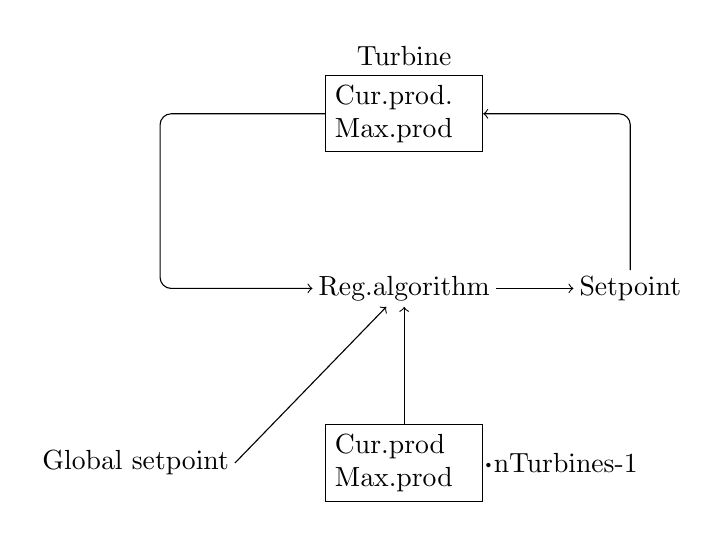
\begin{tikzpicture}[
	point/.style={inner sep=0pt}, %circle,minimum size=2pt,fill=red},
	textNode/.style={inner sep=2pt},
	hv path/.style={to path={-| (\tikztotarget)}},
	vh path/.style={to path={|- (\tikztotarget)}},
	skip loop h/.style={to path={-- ++(0,#1) -| (\tikztotarget)}},
	skip loop v/.style={to path={-- ++(#1,0) |- (\tikztotarget)}},
	graphs/every graph/.style={edges=rounded corners}
	]
	
% Place nodes
\matrix[row sep=1.5cm,column sep=.5cm] {
	\node [point]  		(p1x1)	{}; &&
	\node [rectangle]	(Turbine)		[draw, label=above:Turbine, text width=50pt]	{Cur.prod. Max.prod}; &&
	\node [point]  		(p1x3)	{}; \\
	
	\node [point]  		(p2x1)			{}; &&
	\node [textNode]	(HPPP)		 	{Reg.algorithm}; &&
	\node [textNode]	(Setpoint)	{Setpoint}; \\

	\node [textNode]  (gSetpoint)										{Global setpoint}; &&
	\node [rectangle]	(Data)			[draw, text width=50pt] {Cur.prod  Max.prod};\\
};

\node [textNode,right of=Data] {~~~~~~~~~~~~~~~~~\textbf{$\cdot$}nTurbines-1};
	
\graph[use existing nodes]{
	Turbine ->[skip loop v=-3.1cm] HPPP -> Setpoint ->[vh path] Turbine;
	gSetpoint.east -> HPPP;
	Data -> HPPP;
};

\end{tikzpicture}

	\captionsetup{format=plain,font=footnotesize,labelfont={bf,defaultCapFont},labelsep=quad,singlelinecheck=no}
	\caption[Decentralized input/output parameters of the regulation algorithm]{
		\label{fig:ioDecenRegAlg} 
		\footnotesize{%
			Decentralized input/output parameters of the regulation algorithm.
		}
	}
\end{figure}

The regulation algorithm is now computed on every turbine instead of computing the algorithm on a central Park Pilot. Thus, instead of requesting all states (current production and max production) externally, the regulation algorithm now collects one state from the local turbine. Furthermore the regulation algorithm only calculates a single setpoint - the setpoint used by the local turbine to set a new state - instead of calculating a setpoint for every turbine in the wind farm.

As \cref{fig:ioDecenRegAlg} implies, with the regulation algorithm performed on every turbine, decentralizing the Park Pilot onto the turbines also means that every turbine must know the state of every other turbine in the wind farm.

\section{Regulation cycle}

Decentralizing the Park Pilot onto the turbines has changed the regulation cycle too. The decentralized solution has been built with focus on scalability, in terms of increasing the number of turbines does not impact the regulation cycle, as well as performance, in terms of decreasing the regulation cycle time.

The following sections presents the decentralized regulation cycle. First by describing how the decentralized regulation cycle differs from the centralized regulation cycle, followed by a detailed description of how a single regulation cycle has been implemented. 

%Finally the term \textit{cache reads} is discussed, which is introduced by the decentralized by a discussion of the introduction of cache reads.

\subsection{Changes compared to the centralized regulation cycle}\label{sec:regCycleChanges}

The difference between the centralized regulation cycle and the decentralized regulation cycle is illustrated in \cref{fig:cycleCentralVSDecentral}. 

\begin{figure}[!h]
	%The figure show how regulation time differs central vs decantral

	{\sffamily{Centralized regulation cycle}}
	\newline
	

{ %The brackets issolate the enviroment

\tikzstyle{line}		 	= [draw]

\makeatletter
\ifcsname c@wavenum\endcsname %Only create one counter
\else
	\newcounter{wavenum}
\fi
\makeatother

\newcommand*{\bitvector}[3]{
  \draw[fill=#3] (t_cur) -- ++( .1, .3) -- ++(#2-.2,0) -- ++(.1, -.3)
                         -- ++(-.1,-.3) -- ++(.2-#2,0) -- cycle;
  \path (t_cur) -- node[anchor=mid](textNode) {#1} ++(#2,0) node[time] (t_cur) {};
  }

% \known{val}{length}
\newcommand*{\known}[2]{
    \bitvector{#1}{#2}{white}
}

% \unknown{length}
\newcommand*{\unknown}[2]{
    \bitvector{#1}{#2}{black!20}
}

% \nextwave{name}
\newcommand{\nextwave}[1]{
  %\path (0,\value{wavenum}) node[time] (t_cur) {};
   \path (0,\value{wavenum}) node[left] {#1} node[time] (t_cur) {};
  \addtocounter{wavenum}{-1}
}

\newcommand{\timeSpanLabel}{
	\node (CycleTimeLabel) [rectangle, above = 0.7cm of textNode, inner sep=0pt] {Regulation cycle time};	  
}

\newcommand{\timeSpanA}{
	\node (t_timeSpanA) [point, above = 0 of t_cur] {};	  
}

\newcommand{\timeSpanB}{
	\node (t_timeSpanB) [point, above =0 of t_cur] {};

  \graph[use existing nodes]{
  	t_timeSpanA --[time span=1cm] CycleTimeLabel;
   	CycleTimeLabel.south --[time span=-0.24cm] t_timeSpanB;
  }; 
    	
}


%%% End of timing.sty
\begin{tikzpicture}[
	point/.style={inner sep=0pt}, %circle,minimum size=2pt,fill=red},
	draw=black, 
	yscale=.8,
	xscale=1,
	hv path/.style={to path={-| (\tikztotarget)}},
	vh path/.style={to path={|- (\tikztotarget)}},
	skip loop v/.style={to path={-- ++(#1,0) |- (\tikztotarget)}},		
	skip loop h/.style={to path={-- ++(0,#1) -| (\tikztotarget)}},
	time span/.style={to path={-- ++(0,#1) -| (\tikztotarget)}},
	graphs/every graph/.style={edges=rounded corners}	
	]
	
  \tikzstyle{time}=[coordinate]
  \setlength{\unitlength}{1cm}
  \setcounter{wavenum}{0}
    
  %\nextwave{Regulation Time} \unknown{SendData}{2} \known{WaitForData}{5} \unknown{ReciveData}{2} \unknown{Calculate}{2}\unknown{SendSP}{2}
  \nextwave{Park Pilot} \unknown{reqStates}{1.8} \known{wait}{2} \unknown{readStates}{2} \unknown{regAlg.}{1.7} \unknown{sendSetpoints}{2.6}
  
  \nextwave{Turbine} \known{wait}{1.8} \unknown{replyState}{2} \known{wait}{6.3} \unknown{receiveSetpoint}{2.9}
    
  
\end{tikzpicture}
}

	\newline
	
	{\sffamily{Decentralized regulation cycle (with parallel reception of data)}}
	\newline
	

{ %The brackets issolate the enviroment

\makeatletter
\ifcsname c@wavenum\endcsname %Only create one counter
\else
	\newcounter{wavenum}
\fi
\makeatother

\newcommand*{\bitvector}[3]{
  \draw[fill=#3] (t_cur) -- ++( .1, .3) -- ++(#2-.2,0) -- ++(.1, -.3)
                         -- ++(-.1,-.3) -- ++(.2-#2,0) -- cycle;
  \path (t_cur) -- node[anchor=mid](textNode) {#1} ++(#2,0) node[time] (t_cur) {};
}

% \known{val}{length}
\newcommand*{\known}[2]{
    \bitvector{#1}{#2}{white}
}

% \unknown{length}
\newcommand*{\unknown}[2]{
    \bitvector{#1}{#2}{black!20}
}

% \nextwave{name}
\newcommand{\nextwave}[1]{
  %\path (0,\value{wavenum}) node[left] {#1} node[time] (t_cur) {};
  %\path (0,\value{wavenum}) node[time] (t_cur) {};
  \path (0,\value{wavenum}) node[below left] {#1} node[time] (t_cur) {};
  \addtocounter{wavenum}{-1}
}


\newcommand{\timeSpanA}{
	\node (t_timeSpanA) [point, above = 0 of t_cur] {};	  
}

\newcommand{\timeSpanB}{
	\node (t_timeSpanB) [point, above =0 of t_cur] {};
	
	\graph[use existing nodes]{
		t_timeSpanA --[time span=1cm] CycleTimeLabel;
		CycleTimeLabel.south --[time span=-0.24cm] t_timeSpanB;
	}; 
	
}

%%% End of timing.sty

\begin{tikzpicture}[
	point/.style={inner sep=0pt}, %circle,minimum size=2pt,fill=red},
	draw=black, 
	yscale=.8,
	xscale=1,
	hv path/.style={to path={-| (\tikztotarget)}},
	vh path/.style={to path={|- (\tikztotarget)}},
	skip loop v/.style={to path={-- ++(#1,0) |- (\tikztotarget)}},		
	skip loop h/.style={to path={-- ++(0,#1) -| (\tikztotarget)}},
	time span/.style={to path={-- ++(0,#1) -| (\tikztotarget)}},
	graphs/every graph/.style={edges=rounded corners}	
]
	
\tikzstyle{time}=[coordinate]
\setlength{\unitlength}{1cm}
\setcounter{wavenum}{0}

	\nextwave{Turbine} \unknown{readStates}{2.5} \unknown{regAlg.}{2.5} \unknown{setSetpoint}{2.5} \unknown{sendState}{2.5} \known{sleep}{2}
	\nextwave{} \known{reciveStates}{12}
\end{tikzpicture}
}

	\caption{Centralized vs decentralized regulation cycle}
	\label{fig:cycleCentralVSDecentral}
\end{figure}

In the centralized solution a request for data and waiting for the corresponding reply for every turbine was a requirement for the Park Pilot, turbines in the decentralized solution publish new states whenever a new setpoint has been calculated. Turbines publishes to a specific Topic and are assigned a unique keys. Receiving states from other turbines is handled and loaded asynchronously into memory by Connext, thus receiving states is a parallel process running alongside the regulation algorithm.
This enables a \textit{Distributed Shared Memory (DSM)} (see \cref{sec:DSM} for DSM description) behavior for the decentralized solution, where the state of every turbine is shared with every other turbine in the wind farm.
As every turbine has a unique Topic key, each turbine has assigned its own shared memory space, where only the turbine is allowed to write, as illustrated in \cref{fig:DSMlikeBehavior}, thus removing the possibility that turbines overwrite each others states. Using DSM like behavior for the decentralized solution, means that receiving states from other turbines is abstracted away from the regulation cycle, enabling the turbines to assume that the latest state of every other turbine has been received and is available locally in memory. This alleviates the need for the request-reply part of the centralized regulation cycle. The expectation is that removing the request-reply part of the algorithm decreases the regulation cycle time, since acquisition of turbine states are no longer a part of the regulation cycle.  

\begin{figure}[!h]
	\begin{tabular}{ | c | c | c | c | c |}
		\cline{1-3}
		\cline{5-5}
		turbine 1 & turbine 2 & turbine 3 & \dots & turbine n \\
		\cline{1-3}
		\cline{5-5}
	\end{tabular}
	\caption{Distributed Shared Memory like behavior of the decentralized solution}
	\label{fig:DSMlikeBehavior}
\end{figure}

Removing the request-reply part of the regulation cycle for the decentralized solution, also removes the ability to ensure that regulation happens using latest states only, since a given turbine, when initiating the regulation cycle, reads the turbine states that is already in memory, instead of requesting all the latest states. This of course forces a redefinition of when a state is usable for regulation. Instead of using latest states only, the decentralized solution defines a time limit that, when reached, changes the status of the state to old and thus not usable for regulation. Thus for the decentralized solution it is acceptable to perform regulation using states that are no older than the specified time limits. 

To further decrease the regulation cycle time, strictly reliable messaging has been removed from the decentralized solution. A reply from all turbines at a specific point in the regulation cycle is no longer needed, thus package loss will no longer block the regulation cycle. Furthermore, with the time limit introduced, all states are no longer needed by every turbine, since states now only have to be strictly 'younger' than the specified time limit.
Instead of strictly reliable messaging the decentralized solution use best effort messaging, where data samples are sent once and missed samples are acceptable. As every turbine of the decentralized solution only relies on the newest published state and not every state published, a dropped state is no longer critical as it is overwritten by the state of the next regulation cycle for a given turbine.

Finally multicast has been enabled for the decentralized solution to greatly reduce the number of packages each turbine sends, when publishing a new state. With multicast enabled only one package is sent pr. new state, as opposed to the centralized solution which sends a package per receiver. This reduces the load of each turbine and decreases the regulation cycle time. Furthermore, this also reduces overall network traffic.  

Each turbine only calculate it's own setpoint. Thus after calculation, the new setpoint is set locally and the new state is published to the other turbines. The wait time at the end of the regulation cycle is needed in order to leave a small amount of time for Connext to receive and overwrite states that have already been read.

\subsection{Implementation}

Before running the regulation cycle illustrated in \cref{fig:decenRegCycle}, an initial setpoint is set and the corresponding state of the turbine is read, enabling publishing of the turbine state as the first step of the regulation cycle. This is done to prevent the first cycle from being redundant due to lack of data from other turbines. 

\begin{figure}[!h]
	\centering
	\begin{sequencediagram} %Created using pgf-umlsd
		\newthread{parkPilot}{:Park Pilot}
		\newinst[2]{turbine}{:Turbine}
		\newinst[2]{connext}{:Connext}
		
		\begin {messcall}{parkPilot}{publishState()}{connext}{}
		\end {messcall}
		\begin {call}{parkPilot}{readStates()}{connext}{states}
		\end {call}
		\begin {callself}{parkPilot}{regAlgorithm()}{setpoint}
		\end {callself}
		\begin {call}{parkPilot}{sendSetpoint()}{turbine}{setpoint}
		\end {call}
		\begin {call}{parkPilot}{readState()}{turbine}{state}
		\end {call}	
		\begin {callself}{parkPilot}{sleep()}{}
		\end {callself}			
	\end{sequencediagram}

	\captionsetup{format=plain,font=footnotesize,labelfont={bf,defaultCapFont},labelsep=quad,singlelinecheck=no}
	\caption[Decentralized regulation cycle sequence diagram]{
		\label{fig:decenRegCycle} 
		\footnotesize{%
			Decentralized regulation cycle sequence diagram.
		}
	}
\end{figure}

\Cref{fig:decenRegCycle} presents three objects:

\begin{itemize}
	\item The \textbf{Park Pilot} object which handles the regulation cycle. As opposed to the centralized solution, the Park Pilot object is now instantiated on every turbine in the wind farm, instead of being a single external component.
	\item The \textbf{Turbine} object which serves as the interface to the underlying Turbine. The Turbine object for the purpose of this thesis is just a simulation of an actual turbine. Thus this object handles communication with a database with actual turbine data provided by Siemens Wind Power.
	\item \textbf{Connext} is the underlying DDS framework used for communication, thus this is not an object instantiated by the Park Pilot. It is however what enables reception of data in parallel with the regulation cycle. 
\end{itemize}

The Park Pilot publishes the state of the present turbine and reads the states of every turbine within the wind farm. Afterwards the regulation algorithm is performed and a setpoint for the present turbine is calculated and used to set a new state.

The regulation algorithm used for the decentralized solution is the same used for the centralized solution described in \cref{sec:calculateSetpoints}, with the exception that the setpoint calculated is kept for local purposes instead of sending the setpoint to all turbines. The regulation algorithm code for the decentralized solution is presented in \cref{fig:decenRegAlgCode}.

\begin{figure}[!h]
	\centering
%	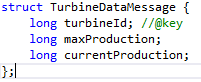
\includegraphics[width=0.3\textwidth,natwidth=250,natheight=200]{turbineDataMessage.PNG} 
	\begin{lstlisting}[language=C++,tabsize=2,basicstyle=\small]
uint_fast32_t DecentralizedParkPilot::regAlgorithm(
	uint_fast32_t globalSetpoint,
	TurbineMessageSeq turbines,
	uint_fast32_t maxProd,
	uint_fast32_t currentProd,
	uint_fast32_t setPoint,
	DDS_SampleInfoSeq turbineInfos,
	uint_fast32_t &cacheCount )
{
	cacheCount = 0;
	if (currentProd >= maxProd)
		return maxProd;

	int availableTurbinesCount = turbines.length();

	for (int i = 0; i < turbines.length(); i++)
	{
		if (!turbineInfos[i].valid_data) {
			availableTurbinesCount--;
			continue;
		}

		if (turbineInfos[i].sample_state == DDS_READ_SAMPLE_STATE) {
			cacheCount++;
		}

		if (turbines[i].currentProduction >= turbines[i].maxProduction)
			availableTurbinesCount--;
	}
	uint_fast32_t localSetpoint = 0;

	if (availableTurbinesCount <= 0)
		localSetpoint = globalSetpoint;
	else
		localSetpoint = globalSetpoint / availableTurbinesCount;

	if (localSetpoint > maxProd) {
		localSetpoint = maxProd;
	}

	return localSetpoint;
}
	\end{lstlisting}
	\captionsetup{format=plain,font=footnotesize,labelfont={bf,defaultCapFont},labelsep=quad,singlelinecheck=no}
	\caption[The regulation algorithm of the decentralized solution]{
		\label{fig:decenRegAlgCode} 
		\footnotesize{%
			Code for the decentralized regulation algorithm used to calculate setpoints.
		}
	}
\end{figure}

\subsection{Cache reads}\label{sec:cachereads}

A cache read happens if the cycle time elapses before all turbine instances have responded with state information, resulting in the same state being read twice. Thus it is a natural result of separating receiving data from the regulation cycle, as done in the decentralized solution. Connext only keeps track of data that has already been read but not how many times that data has been read. Thus a cache read does not include information regarding if the same state has been read multiple times.

The regulation cycle of the decentralized solution does not directly include any communication, thus enabling a significant reduction of regulation cycle time. However, decreasing the cycle time, increases the 'pressure' on Connext by increasing the number of regulation cycles pr. minute, thus increasing the number of states that needs to be published, thus increasing the number of states that needs to be received (assuming that the cycle time of all turbines are equally decreased). This ultimately results in increased number of cache reads and increased network traffic. Thus decreasing the regulation cycle time will increase the number of cache reads.  

Increasing the number of cache reads can be an issue, since it reduces the effectiveness of the regulation cycle. Having a high number of cache reads implies that the regulation has been performed using data used for the previous regulation, thus decreasing the effect of the current regulation.

As a result of this trade-off between reduction in regulation cycle time and number of cache reads, a sleep is introduced at the end of the regulation cycle (as presented in \cref{fig:decenRegCycle}), in order to control the reduction of the regulation cycle. Thus the regulation cycle time is an input parameter of the decentralized solution.

\section{DDS configuration} \label{sec:decen:ddsconf}

The key component used for communication is DDS (see \cref{sec:DSM} for DDS description). This section describes how DDS has been configured for the decentralized solution.

\subsection{Interface Definition Language}\label{sec:decenIdl}

As with the centralized solution, Interface Definition Language (IDL) has been used for generating Data Transfer Objects for the decentralized solution. See centralized IDL \cref{sec:cenIdl} for details.

\begin{figure}[!h]
	\centering
	%	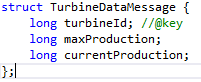
\includegraphics[width=0.3\textwidth,natwidth=250,natheight=200]{turbineDataMessage.PNG} 
	\begin{lstlisting}[language=C++,tabsize=2,basicstyle=\small]
	struct TurbineMessage {
		long turbineId; //@key
		long maxProduction;
		long currentProduction;
		long setPoint;
		long msSinceLastWrite;
		long cacheCount;
	};	
	\end{lstlisting}
	\captionsetup{format=plain,font=footnotesize,labelfont={bf,defaultCapFont},labelsep=quad,singlelinecheck=no}
	\caption[Decentralized turbine message]{
		\label{fig:decenTurbineMessage} 
		\footnotesize{%
			The turbine message .idl file sent from the turbines to all other turbines in the decentralized solution.
		}
	}
\end{figure}

\subsection{Choosing Quality of Service parameters}\label{sec:decenChoosingQoS}

The Quality of Service (QoS) parameters for the decentralized solution is based on the QoS parameters determined for the centralized solution, except for the following key areas:

\begin{description}
	\item[Reliability] of messaging has been changed to best effort messaging in order to reduce the regulation cycle time. This means package drops are allowed for the decentralized solution.
	\item[Durability] of the decentralized solution has been changed to local durability. This means that the current state of every turbine is sent to newly discovered turbines. Note that with best effort messaging there is no guarantee that the states are received, since package drops are allowed. Durability for the regulation cycle has only minor relevance, since newly arrived turbines will receive all states within a short amount of time after being discovered. Thus this setting has only been applied, since an attempt to receive states upon startup is better than receiving no states at all. However, for real life purposes, the turbines should probably be configured with a default setpoint, which is used until data from all turbines has been received, in combination with this setting. 
	\item[Throughput] remains the same as the throughput setting of the centralized solution but for a slightly different reason. New turbine states must be sent as soon as possible, which removes the need for batching. \todo{Hvorfor gør det batching irrelevant?} Thus regular throughput has been chosen for the decentralized solution. 
	\item[Multicast] has been enabled to reduce regulation cycle time and network traffic, as explained in \cref{sec:regCycleChanges}.
\end{description}

\subsection{Detailed quality of service evaluation}

This section provides a detailed evaluation of every parameter used for the decentralized QoS XML. The full QoS XML is presented but only parameter changes from the centralized solution are discussed.

\paragraph{Participant factory} (\cref{fig:decParFacQos}) QoS parameters has been set to be the same as the centralized solution. See Participant factory description of \cref{sec:detailedQoSDesc}.

\begin{figure}[!h]
\begin{lstlisting}[language=XML]
<participant_factory_qos>
	<logging>
		<verbosity>WARNING</verbosity>
		<category>PLATFORM</category>
		<print_format>VERBOSE_TIMESTAMPED</print_format>
		<output_file>ddsadaptor.log</output_file>
	</logging>
</participant_factory_qos>
\end{lstlisting}
\caption[Decentralized participant factory QoS parameters]{
		\label{fig:decParFacQos} 
		\footnotesize{Participant factory QoS parameters of the decentralized solution.}
	}
\end{figure}

\paragraph{Participant} (\cref{fig:decParQos}) QoS parameters has been evaluated as follows (see Participant evaluation of \cref{sec:detailedQoSDesc} for parameters not described):

\begin{itemize}
	\item \textbf{.builtin.multicast\_enabled} value has been set to 1 to enable multicast.
\end{itemize}

\begin{figure}[!h]
\begin{lstlisting}[language=XML]
<participant_qos>
	<participant_name>
		<name>TurbineParticipant</name>
		<role_name>TurbineParticipantRole</role_name>
	</participant_name>
		<database>
		<shutdown_cleanup_period>
			<sec>DURATION_ZERO_SEC</sec>
			<nanosec>1</nanosec>
		</shutdown_cleanup_period>
	</database>
		<transport_builtin>
			<mask>UDPv4</mask>
		</transport_builtin>
	<property>
		<value>
			<element>
				<name>dds.transport.UDPv4.builtin.multicast_enabled</name>
				<value>1</value>
			</element>
			<element>
				<name>dds.transport.UDPv4.builtin.parent.message_size_max</name>
				<value>65535</value>
			</element>
			<element>
				<name>dds.transport.UDPv4.builtin.send_socket_buffer_size </name>
				<value>65535</value>
			</element>
			<element>
				<name>dds.transport.UDPv4.builtin.recv_socket_buffer_size</name>
				<value>2097152</value>
			</element>
		</value>
	</property>
</participant_qos>
\end{lstlisting}
\caption[Decentralized participant QoS parameters]{
		\label{fig:decParQos} 
		\footnotesize{Participant QoS parameters of the decentralized solution.}
	}
\end{figure}

\paragraph{Topic} (\cref{fig:decTopicQos}) QoS parameters are used to initialize DataReader and DataWriter QoS paramters. Thus parameters that applies to both DataReaders and DataWriters have been configured using a Topic profile. Topic QoS parameters have been evaluated as follows:

\begin{itemize}
	\item \textbf{reliability} of the decentralized solution has been set to best effort, as discussed in \cref{sec:decenChoosingQoS}, thus making package drops acceptable.
	\item \textbf{durability} has been set to local durability, thus latest states from all online turbines are sent to newly added turbines.
	
	Note that in combination with best effort reliability, a newly added turbines is not ensured all turbine states. Furthermore the amount of states received from each turbines is the depth value set by the history QoS parameter.
	\item \textbf{history} configures the number of data samples the send and receive buffers can contain on a per instance basis for keyed Topics. With KEEP\_LAST\_HISTORY\_QOS enabled, the latest values of the data samples are kept and old samples are discarded when the limit as set by the depth parameter is reached. Thus the send and receive buffers of the decentralized solution acts like a circular buffer of length 1, meaning, in combination with best effort messaging, only newest states are available to the turbines.
\end{itemize}

\begin{figure}[!h]
\begin{lstlisting}[language=XML]
<topic_qos name="TurbineTopicQos">
	<reliability>
		<kind>DDS_BEST_EFFORT_RELIABILITY_QOS</kind>
	</reliability>
	<durability>
		<kind>TRANSIENT_LOCAL_DURABILITY_QOS</kind>
	</durability>
	<history>
		<kind>KEEP_LAST_HISTORY_QOS</kind>
		<depth>1</depth>
	</history>
</topic_qos>
\end{lstlisting}
\caption[Decentralized Topic QoS parameters]{
		\label{fig:decTopicQos} 
		\footnotesize{Topic QoS parameters of the decentralized solution.}
	}
\end{figure}

\paragraph{DataWriter} (\cref{fig:decDataWriterQos}) QoS parameters has been evaluated as follows (see DataWriter evaluation of \cref{sec:detailedQoSDesc} for parameters not described):

\begin{itemize}
	\item \textbf{lifespan} configures the expiration time of each data sample written by a DataWriter. Thus this parameter is only relevant to DataWriters. Each data sample has an associated expiration time, beyond which the data should not be delivered. Once the sample expires, the data sample will be removed from the DataReaders receive buffers. 
	
	This parameter configures the previously mentioned time limit (\cref{sec:regCycleChanges}) of the decentralized solution. A turbine state expires after 150000000 nanoseconds ($=150$ ms). This value is set after the worst case regulation cycle time of the current Siemens system, to ensure that the decentralized solution do not use data older than what the current Siemens system use for regulation.
	
	Furthermore, this parameter also indirectly controls how many and which turbines should be used for the regulation algorithm. If a state is older than 150 ms, the state is automatically removed from the receive buffer, thus it is removed from the data that is read and used for the regulation algorithm. As the regulation algorithm automatically scales with the number of turbines, from which a state has been received within the latest 150 ms, the turbine which have not sent a new state within 150 ms will be considered offline. For this reason the lifespan parameter is responsible for the tolerance of the decentralized solution. If a turbines fails, the state of the turbine will eventually expire, thus removing the turbine from the regulation algorithm.
\end{itemize}

\begin{figure}[!h]
\begin{lstlisting}[language=XML]
<datawriter_qos>
	<publication_name>
		<name>TurbineDataWriter</name>
	</publication_name>
	<lifespan>
		<duration>
			<sec>0</sec>
			<nanosec>150000000</nanosec>
		</duration>
	</lifespan>
</datawriter_qos>
\end{lstlisting}
\caption[Decentralized DataWriter QoS parameters]{
		\label{fig:decDataWriterQos} 
		\footnotesize{DataWriter QoS parameters of the decentralized solution.}
	}
\end{figure}

\paragraph{DataReader} (\cref{fig:decDataReaderQos}) QoS parameters has been evaluated as follows (see DataReader evaluation of \cref{sec:detailedQoSDesc} for parameters not described):

\begin{itemize}
	\item \textbf{multicast} specifies the multicast addresses on which DataReaders receives data from DataWriters. 
\end{itemize}

\begin{figure}[!h]
\begin{lstlisting}[language=XML]
<datareader_qos>
	<subscription_name>
		<name>TurbineDataReader</name>
	</subscription_name>
	<multicast>
		<kind>AUTOMATIC_TRANSPORT_MULTICAST_QOS</kind>
		<value>
			<element>
				<receive_address>239.192.0.1</receive_address>
			</element>
		</value>
	</multicast>
</datareader_qos>
\end{lstlisting}
\caption[Decentralized DataReader QoS parameters]{
		\label{fig:decDataReaderQos} 
		\footnotesize{DataReader QoS parameters of the decentralized solution.}
	}
\end{figure}
% !TeX spellcheck = en_US

\chapter{Experiments}

\newcommand{\failingTurbineNumbers}{1, 5, 10 and 30}
\newcommand{\testTurbineNumbers}{2, 21, 41, 61, 81 and 101}
\newcommand{\experiemntRunTime}{2mins}


The goal of this project was not only to build a control system that provides both scalability and availability, but also to compare it to the current solution by Siemens Windpower. 
In order to evaluate the system, we have created the experiments in the following sections.

The experiments are done using up to 3 machines connected using a 1Gbit ethernet router with IGMP support.
The experiments are run on 3 laptops, with one being used to capture test data and the other 2 optionally running a number of turbines controllers to generate traffic.
All test are run with CPU utilization on average below 90\%, this is done to keep performance consistent.
The specification of the hardware used for testing can be found in \cref{appendix:HardwareSpecification}.
Every experiment is run at least X times 

\section{PS \ref{PS:Q:CanWeDoIt}: Does our prototype work?}
We start the prototype:
\begin{itemize}
	\item Does it communicate without a central system?
	\item Does the sum of the turbines setpoints match the global setpoint? 
\end{itemize}

\section{PS \ref{PS:Q:Availlability}: Fault tolerance of the system}

The below experiment is done with a variating N number of failing turbines \failingTurbineNumbers.
The experiment has the following procedure:
\begin{enumerate}
	\item Start the system with 100 turbines.
	\item Make sure the system is stable.
	\item Kill N nodes.
	\begin{itemize}
		\item did the system discover the failed node within a 150ms timeframe?
		\item did the system adjust the setpoints for all turbines to keep the global setpoint correct?
	\end{itemize}
\end{enumerate}


\section{PS \ref{PS:Q:CanWeScale}: Scalability of regulation algorithm}
Scalability is by Bondi\cite{Bondi:2000:CSI:350391.350432} defined as \textit{the systems ability to accommodate an increasing number of elements or objects, to process growing volumes of work gracefully, and/or to be susceptible to enlargement}.

The experiments below are made to show how the number of turbines effect the regulation cycle in the decentralized system described in \cref{cha:decentralizedSystem}.
The tests are done with \testTurbineNumbers ~turbine controllers. Besides turbines we are also going to modify ''Data Wait Time Frame'' witch is a constant that defines the time a turbine controller will wait for new updates before considering the other turbine controller offline and unavailable, i.e. regulation speed.

The test system is expected to be running only one instance in a real life implementation, therefore the test machine will only run one instance and the support machines will run the rest generating system load.
The experiment is done with a variating N number of online turbines.
The following procedure is used each time the experiment is done:
\begin{enumerate}
	\item Start the system with N turbines.
	\item Make sure the system is stable.
	\item Start logging the reported regulation run time and cache read count.
	\item Stop logging after \experiemntRunTime.
\end{enumerate}

\section{PS \ref{PS:Q:HowWellDoWeScale}: Comparing decentralized with centralized}
Theses experiments seek to compare the new decentralized (see \cref{cha:decentralizedSystem}) system with the current centralized Siemens system(see \cref{cha:existingSystem}).

The experiments below are made to show how the number of turbines and regulation speed affect the regulation algorithm, memory consumption and Network traffic.
Each of these parameters behave differently when centralized compared to decentralized as seen in \cref{fig:timingCentralVSDecentral} the decentralized system does not wait for new data before doing calculations. Because of this the decentralized version has a extra parameter witch says how much data was updated before calculation was run.

\begin{figure}[b]
	%The figure show how regulation time differs central vs decantral
	\centering
	{\sffamily{Centralized approach}}
	

{ %The brackets issolate the enviroment

\makeatletter
\ifcsname c@wavenum\endcsname %Only create one counter
\else
	\newcounter{wavenum}
\fi
\makeatother

\newcommand*{\bitvector}[3]{
  \draw[fill=#3] (t_cur) -- ++( .1, .3) -- ++(#2-.2,0) -- ++(.1, -.3)
                         -- ++(-.1,-.3) -- ++(.2-#2,0) -- cycle;
  \path (t_cur) -- node[anchor=mid] {#1} ++(#2,0) node[time] (t_cur) {};
}

% \known{val}{length}
\newcommand*{\known}[2]{
    \bitvector{#1}{#2}{white}
}

% \unknown{length}
\newcommand*{\unknown}[2]{
    \bitvector{#1}{#2}{black!20}
}

% \nextwave{name}
\newcommand{\nextwave}[1]{
  \path (0,\value{wavenum}) node[left] {#1} node[time] (t_cur) {};
  \addtocounter{wavenum}{-1}
}

% \begin{wave}[clkname]{num_waves}{clock_cycles}
\newenvironment{wave}{
  \begin{tikzpicture}[draw=black, yscale=.8,xscale=1]
    \tikzstyle{time}=[coordinate]
    \setlength{\unitlength}{1cm}
    \setcounter{wavenum}{0}
    
}{\end{tikzpicture}}

%%% End of timing.sty

\begin{wave}
 \nextwave{Regulation Time} \unknown{SendData}{2} \known{WaitForData}{5} \unknown{ReciveData}{2} \unknown{Calculate}{2}
\end{wave}
}

	\newline
	
	{\sffamily{Decentralized approach}}
	

{ %The brackets issolate the enviroment

\makeatletter
\ifcsname c@wavenum\endcsname %Only create one counter
\else
	\newcounter{wavenum}
\fi
\makeatother

\newcommand*{\bitvector}[3]{
  \draw[fill=#3] (t_cur) -- ++( .1, .3) -- ++(#2-.2,0) -- ++(.1, -.3)
                         -- ++(-.1,-.3) -- ++(.2-#2,0) -- cycle;
  \path (t_cur) -- node[anchor=mid](textNode) {#1} ++(#2,0) node[time] (t_cur) {};
}

% \known{val}{length}
\newcommand*{\known}[2]{
    \bitvector{#1}{#2}{white}
}

% \unknown{length}
\newcommand*{\unknown}[2]{
    \bitvector{#1}{#2}{black!20}
}

% \nextwave{name}
\newcommand{\nextwave}[1]{
  %\path (0,\value{wavenum}) node[left] {#1} node[time] (t_cur) {};
  \path (0,\value{wavenum}) node[time] (t_cur) {};
  \addtocounter{wavenum}{-1}
}

%\newcommand{\timeSpanLabel}{
%	\node (CycleTimeLabel) [rectangle, above = 0.25cm of textNode, inner sep=10pt] {CycleTime};	  
%}

\newcommand{\timeSpanLabel}{
	\node (CycleTimeLabel) [rectangle, above = 1.02cm of t_cur, inner sep=0pt] {Regulation cycle time};
}

\newcommand{\timeSpanA}{
	\node (t_timeSpanA) [point, above = 0 of t_cur] {};	  
}

\newcommand{\timeSpanB}{
	\node (t_timeSpanB) [point, above =0 of t_cur] {};
	
	\graph[use existing nodes]{
		t_timeSpanA --[time span=1cm] CycleTimeLabel;
		CycleTimeLabel.south --[time span=-0.24cm] t_timeSpanB;
	}; 
	
}

%%% End of timing.sty

\begin{tikzpicture}[
	point/.style={inner sep=0pt}, %circle,minimum size=2pt,fill=red},
	draw=black, 
	yscale=.8,
	xscale=1,
	hv path/.style={to path={-| (\tikztotarget)}},
	vh path/.style={to path={|- (\tikztotarget)}},
	skip loop v/.style={to path={-- ++(#1,0) |- (\tikztotarget)}},		
	skip loop h/.style={to path={-- ++(0,#1) -| (\tikztotarget)}},
	time span/.style={to path={-- ++(0,#1) -| (\tikztotarget)}},
	graphs/every graph/.style={edges=rounded corners}	
]
	
\tikzstyle{time}=[coordinate]
\setlength{\unitlength}{1cm}
\setcounter{wavenum}{0}

	\nextwave{} \timeSpanA \unknown{readStates}{3} \unknown{calculate}{3} \timeSpanLabel \unknown{setSetpoint}{3} \unknown{sendState}{3} \timeSpanB \known{wait}{2}
	\nextwave{} \known{reciveStates}{14}
\end{tikzpicture}
}

	\caption{Centralized vs decentralized regulation time}
	\label{fig:timingCentralVSDecentral}
\end{figure}

	The centralized version is split into two applications a client and a server.
	What we aim to primarily compare here is the regulation therefore the client side of the application is not measured. This means that the decentralized version is at slight disadvantage.
	The following procedure is used each time the experiment is done, the procedure is done with N simulated turbines for both :

\begin{minipage}{\textwidth}
	\begin{enumerate}
		\item Start the system with N turbines.
		\item Make sure the system is stable.
		\item Start logging:
		\begin{itemize}
			\item Reported regulation run time (Central only, Decentralized is reused)
			\item Memory and Bandwidth
		\end{itemize}
		\item Stop logging after \experiemntRunTime.
		\end{enumerate}
\end{minipage}

% !TeX spellcheck = en_US

\chapter{Results}

\section{PS \ref{PS:Q:Feasibility}: Does our prototype work?}
We start the prototype does it communicate with out a central system?

\begin{figure}
	\centering
	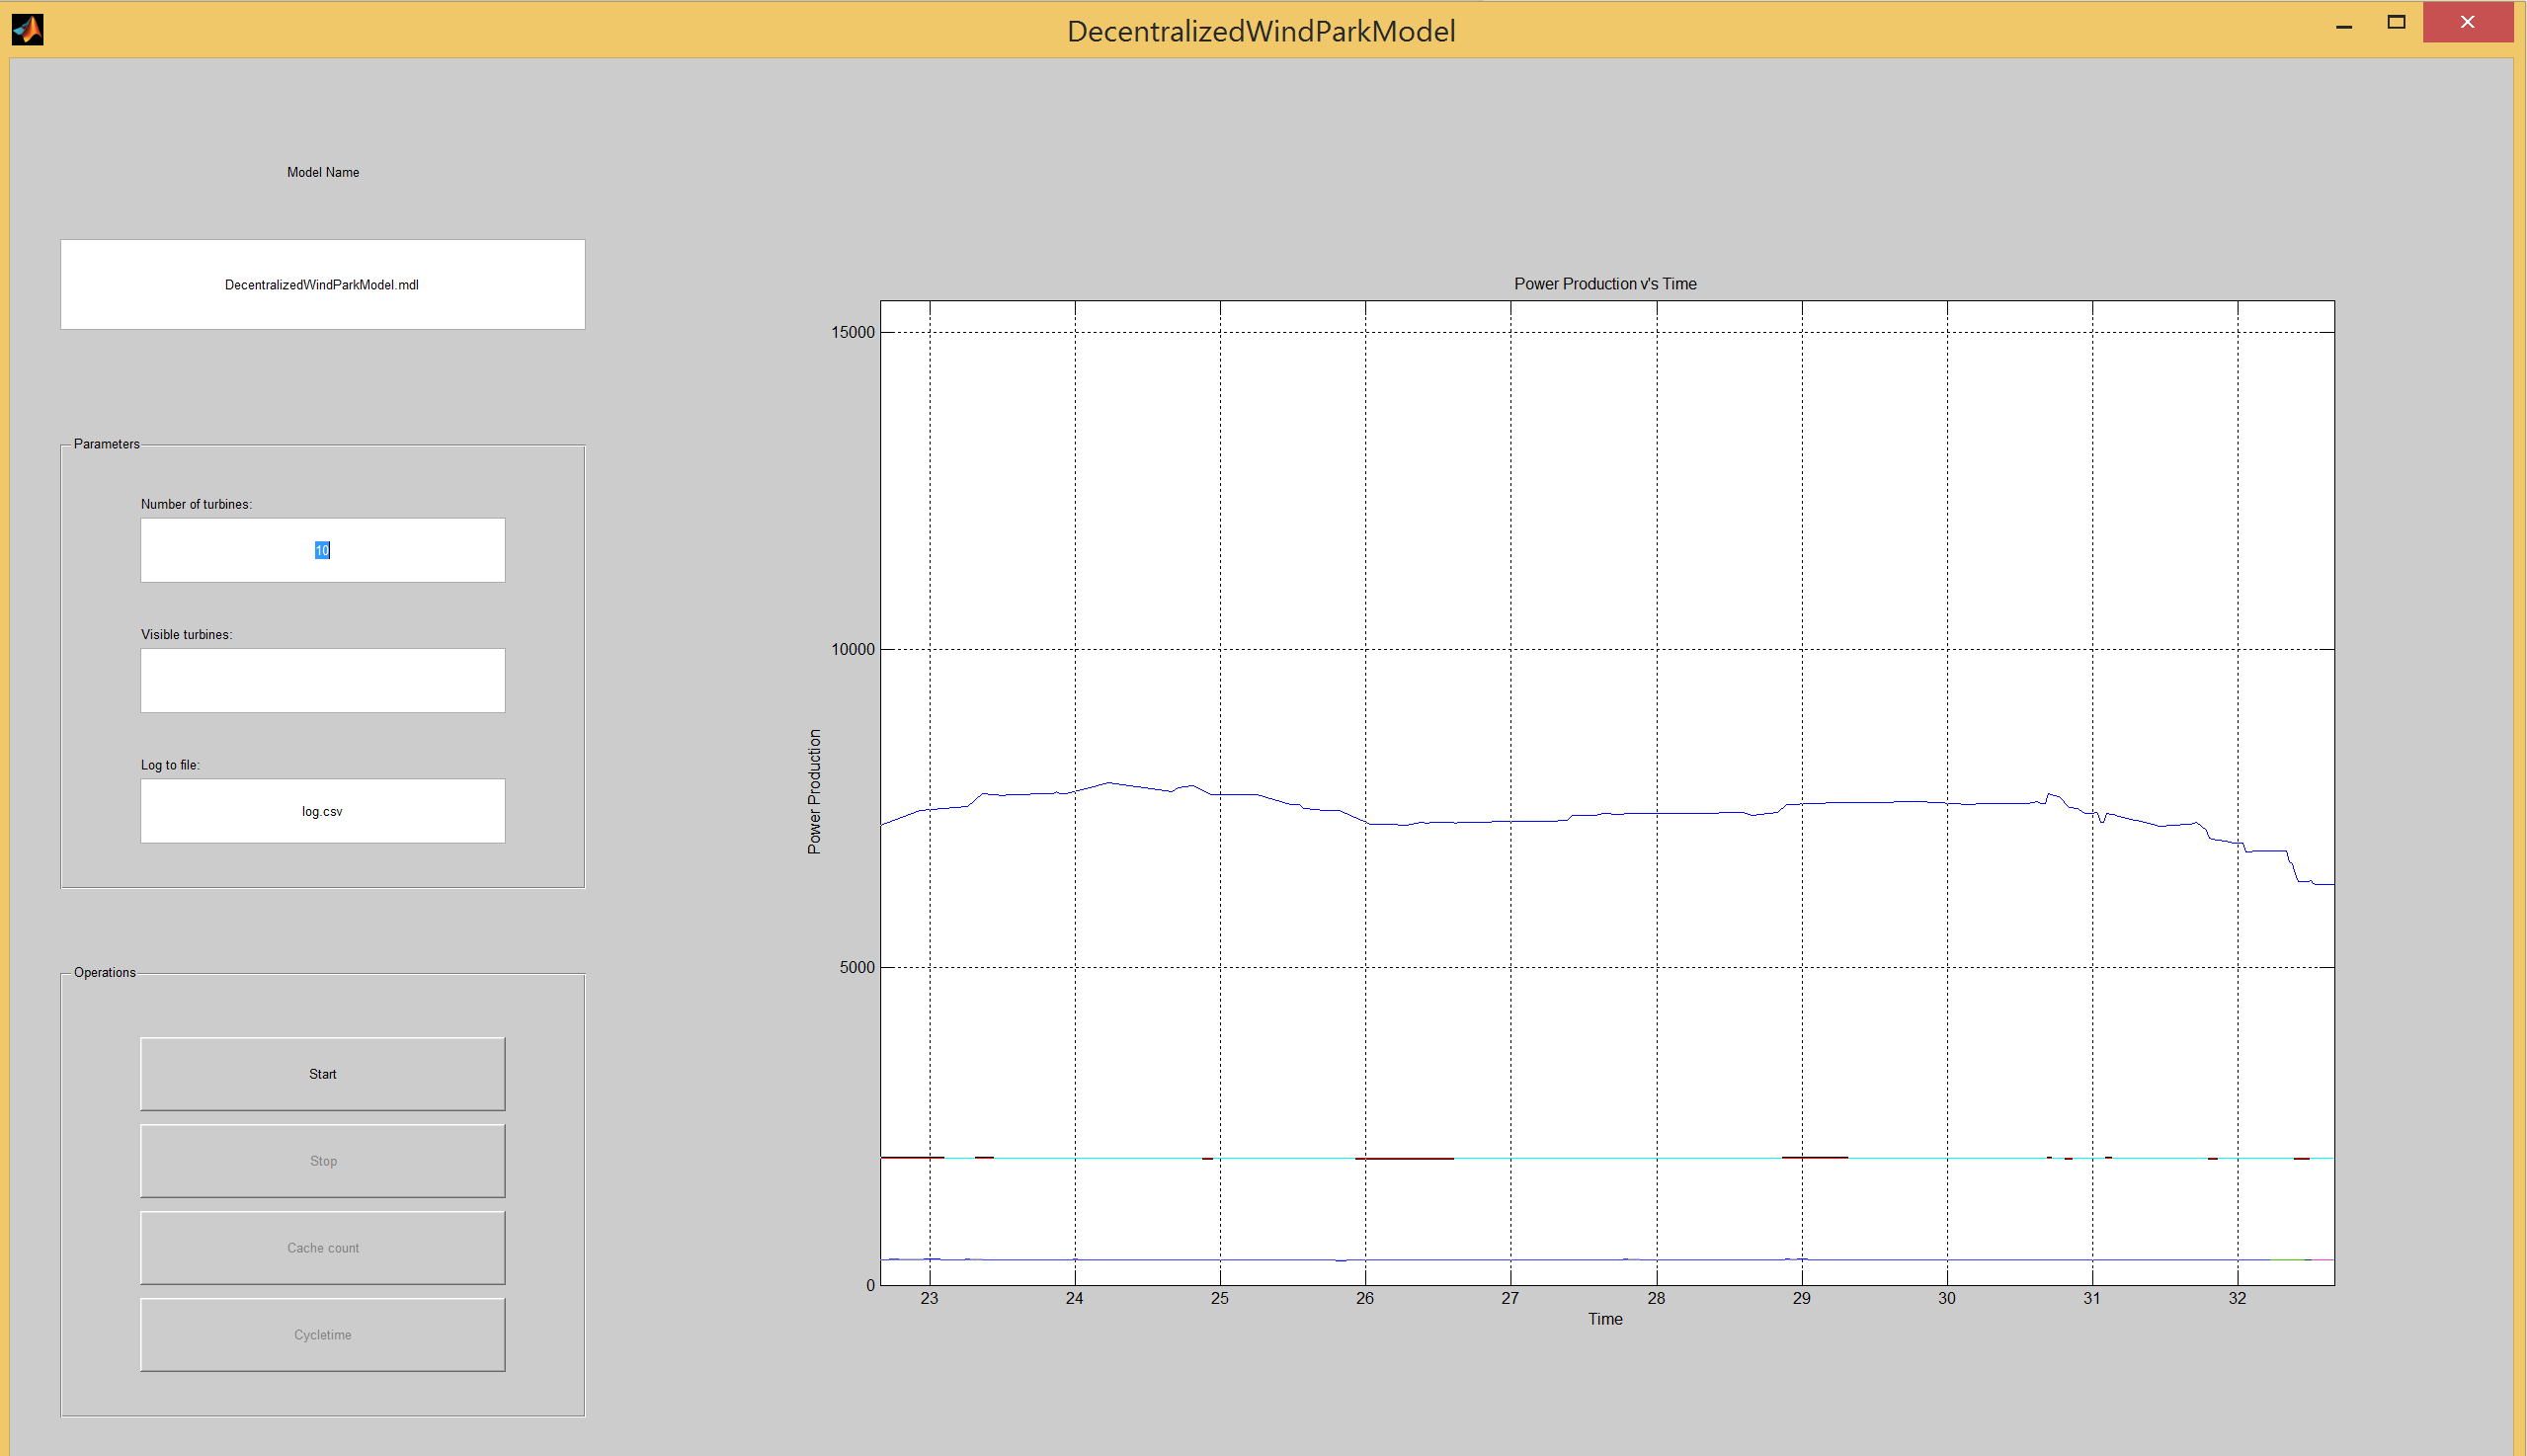
\includegraphics[width=0.9\textwidth,natwidth=610,natheight=642]{gui.png} 
	\captionsetup{format=plain,font=footnotesize,labelfont={bf,defaultCapFont},labelsep=quad,singlelinecheck=no}
	\caption[Graphical interface running 5 turbines]{
		\label{fig:publishSubscribe} 
		\footnotesize{%
			Graphical interface running 5 turbines.
		}
	}
\end{figure}


\section{PS \ref{PS:Q:Availability}: Remove node without system failure?}
Randomly kill client, plot a few seconds of data around the event.

\section{PS \ref{PS:Q:Performance}: Can we make a solution that scales?}

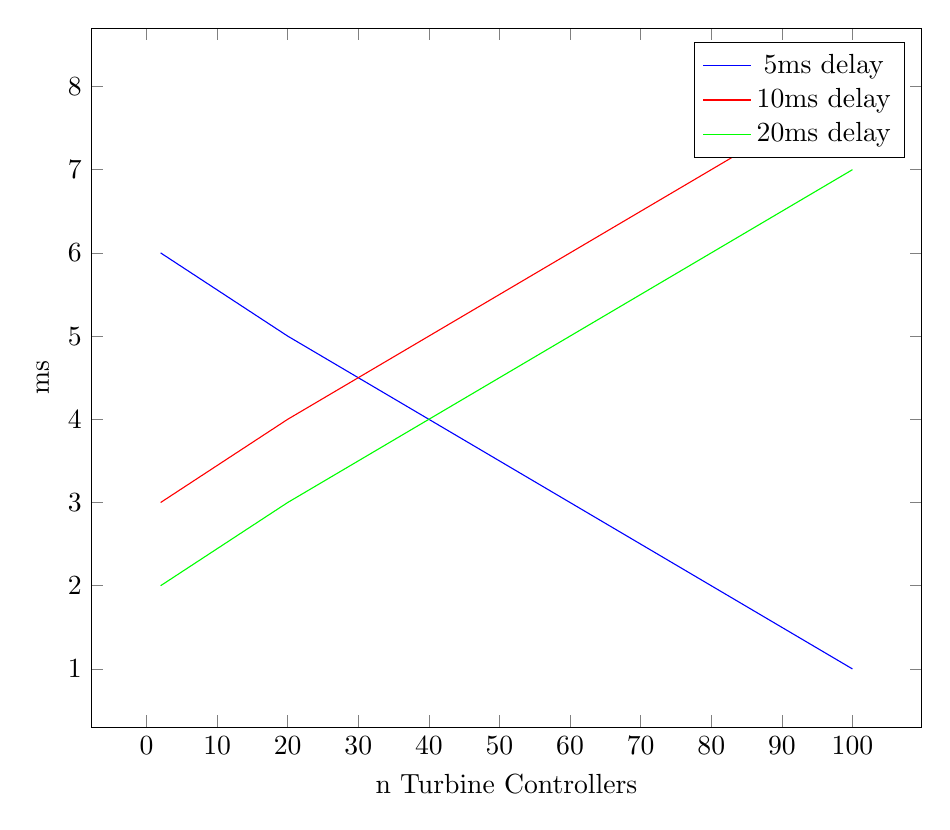
\begin{tikzpicture}
\begin{axis}[
width=\textwidth,
%ymax=0.5,
xlabel=n Turbine Controllers,
ylabel=ms]
\addplot[blue!20!blue] coordinates {
	(2 ,6)
	(20 ,5)
	(40 ,4)
	(60 ,3)
	(80 ,2)
	(100 ,1)
		};
\addplot[red!20!red] coordinates {
	(2 , 3)
	(20 ,4)
	(40 ,5)
	(60 ,6)
	(80 ,7)
	(100,8)	
	};
\addplot[green!20!green] coordinates {
		(2 , 2)
		(20 ,3)
		(40 ,4)
		(60 ,5)
		(80 ,6)
		(100,7)	
	};
\legend{5ms delay,10ms delay,20ms delay}
\end{axis}
\end{tikzpicture}



\section{PS \ref{PS:Q:Scalability}: Does it scale well compared to the centralized version?}
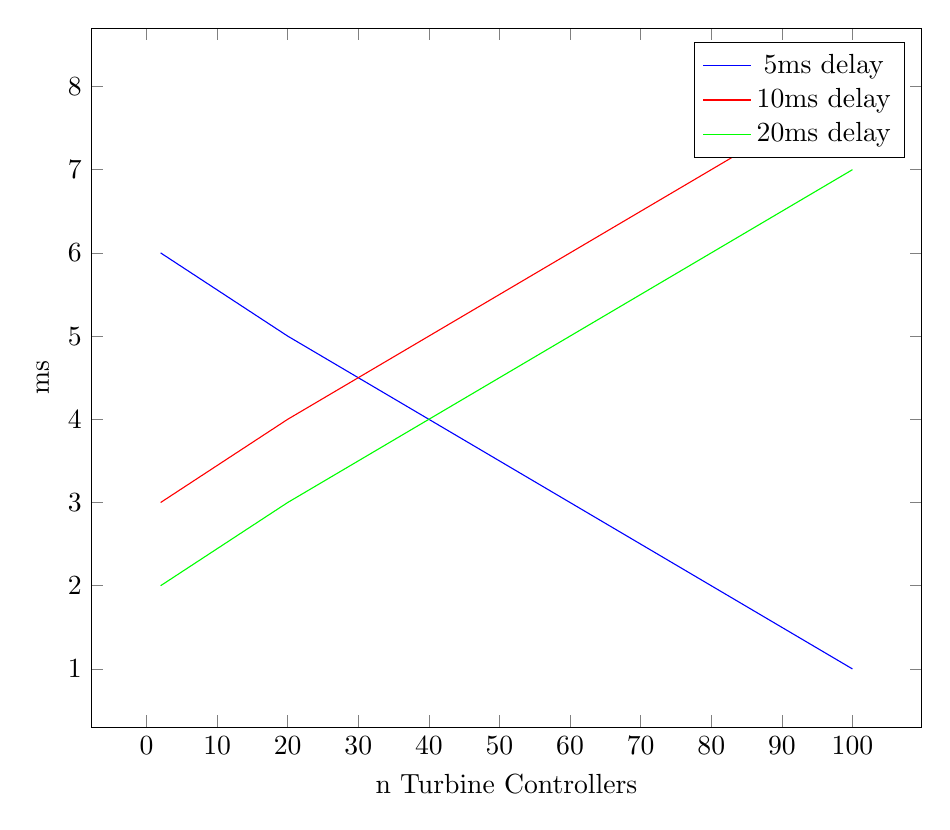
\begin{tikzpicture}
\begin{axis}[
width=\textwidth,
%ymax=0.5,
xlabel=n Turbine Controllers,
ylabel=ms]
\addplot[blue!20!blue] coordinates {
	(2 ,6)
	(20 ,5)
	(40 ,4)
	(60 ,3)
	(80 ,2)
	(100 ,1)
		};
\addplot[red!20!red] coordinates {
	(2 , 3)
	(20 ,4)
	(40 ,5)
	(60 ,6)
	(80 ,7)
	(100,8)	
	};
\addplot[green!20!green] coordinates {
		(2 , 2)
		(20 ,3)
		(40 ,4)
		(60 ,5)
		(80 ,6)
		(100,7)	
	};
\legend{5ms delay,10ms delay,20ms delay}
\end{axis}
\end{tikzpicture}


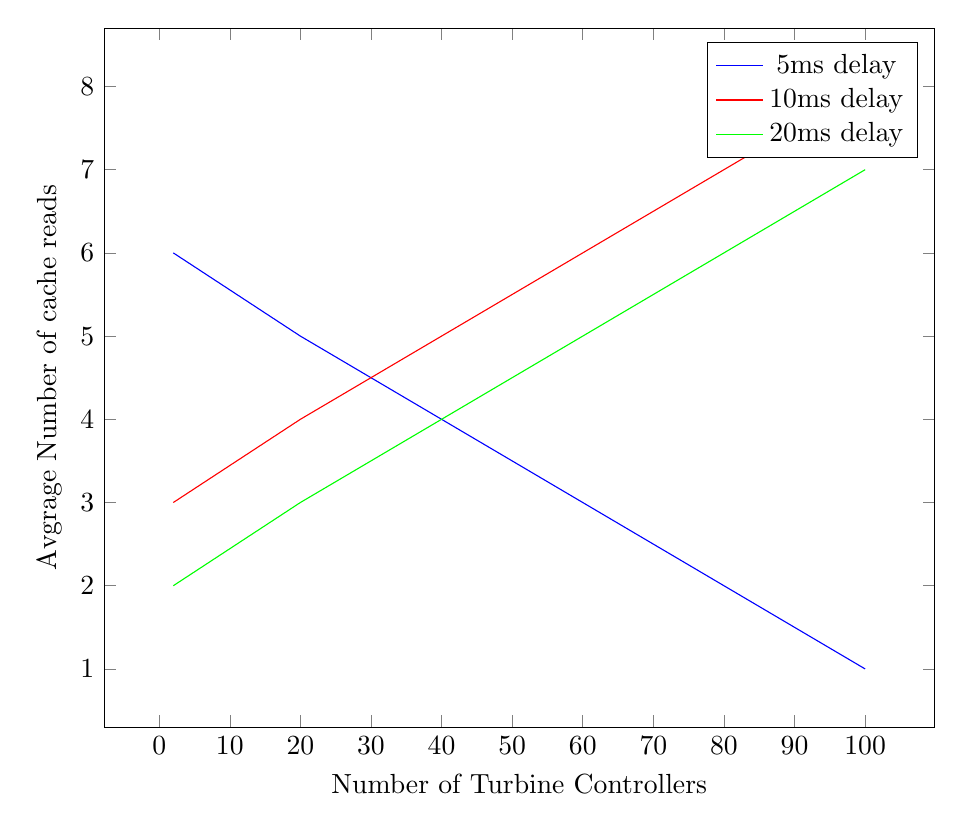
\begin{tikzpicture}
\begin{axis}[
width=\textwidth,
%ymax=0.5,
xlabel=Number of Turbine Controllers,
ylabel=Avgrage Number of cache reads]
\addplot[blue!20!blue] coordinates {
		(2 ,6)
		(20 ,5)
		(40 ,4)
		(60 ,3)
		(80 ,2)
		(100 ,1)
	};
\addplot[red!20!red] coordinates {
		(2 , 3)
		(20 ,4)
		(40 ,5)
		(60 ,6)
		(80 ,7)
		(100,8)	
	};
\addplot[green!20!green] coordinates {
		(2 , 2)
		(20 ,3)
		(40 ,4)
		(60 ,5)
		(80 ,6)
		(100,7)	
	};
\legend{5ms delay,10ms delay,20ms delay}
\end{axis}
\end{tikzpicture}


% !TeX spellcheck = en_US
\chapter{Discussion}

\section{Number of turbines and the impact on regulation cycle time in the decentralized solution}
This section addresses the \ref{PS:Q:Performance} problem of \cref{sec:problemStatement}. In the current Siemens system the regulation cycle time of a single Park Pilot scales linearly with the number of turbines.
The aim of the decentralized solution is to detach the regulation cycle time from being dependent on the number of turbines. 
Looking at \cref{fig:exp:decen:turbines} in \cref{chap:results} we see that the decentralized solution is almost independent on the number of turbines.
From 5 to 65 turbines the regulation cycle time is nearly constant on $20 ms$ with very little variation in the dataset and moderate extreme values.
The constant regulation cycle time is caused by the fact that the regulation cycle in the decentralized system is not forced to wait for data before running the regulation algorithm because data is continually shared between turbines.

When looking at regulation cycle time of the decentralized solution the number cache reads.
As explained in \cref{sec:exp:performance} a cache read happens when a turbine does not provide a new turbine state package before the next regulation cycle is started.
This forces the regulation cycle to use old data read from cache.
Looking at \cref{fig:exp:decen:turbines_cache} we see that the average number of cache reads in the decentralized solution are below 5 and increasing slightly until we reach 65 turbines. From there the number of cache reads increases exponentially.

The increase in regulation cycle time and cache reads when the number of turbines reaches 65 can be explained by the fact that the network equipment of the test setup is approaching maximum throughput capacity which may cause lost or delayed network packages.
Since regulation cycle time in the decentralized system is dependent on the reception time of the oldest turbine state package as explained in \cref{sec:exp:performance} the loss or delay of network packages has a direct impact on regulation cycle time.
Similarly lost or delayed network packages increases the use of cached data. The increased regulation cycle time and cache reads are thus not a limitation of the decentralized solution but a limitation imposed by the test setup.

Disregarding the limitations imposed by the test setup we see that the regulation cycle time is nearly constant while the number of cache reads increases slowly with a factor of around 1 cache read for every 30 turbines added.

The number of cache reads can be reduced by increasing the regulation cycle time as presented in \cref{fig:exp:decen:sleep-cache}.
Thus the factor deciding the time of the regulation cycle is the maximum number of average cache reads accepted for a single regulation cycle.

\section{Comparison of decentralized solution and centralized solution}

\section{Comparison of decentralized and current Siemens system}

\begin{itemize}
	\item Test parameters: Our system vs Siemens system?
	\item Redundancy, up time, scalability...
	\item Solved problems (i.g. Single point of failure)
\end{itemize}
\chapter{Conclusion}


\appendix
\addtocontents{toc}{\protect\setcounter{tocdepth}{0}}
\appendixpage

\chapter{Hardware Specifications}\label{appendix:HardwareSpecification}


\section{D-link DIR-855, Gigabyte Router}



\section{Macbook pro}\label{appendix:hardwareSpecification_pro}

\section{Asus UX32VD}\label{appendix:hardwareSpecification_asus}

\section{Macbook Air}\label{appendix:hardwareSpecification_air}
% include{appendix1}


\backmatter
\renewcommand{\bibsection}{%
\chapter{\bibname}
\prebibhook}
\bibliographystyle{plain} % eller en anden stil
%\bibliographystyle{IEEEbib}
\bibliography{my-bibliography-file}
%\bibliography{minbib}
% print indeks hvis det er noget man anvender

\clearpage
\listoffigures
\clearpage
\listoftables
\chapter{Nomenclature}


\begin{table}[ht]
\captionsetup{singlelinecheck=false,labelsep=newline,justification=centering,font=footnotesize,labelfont={bf,defaultCapFont},format=plain}
\caption[Nomenclature]{\textsc{\ann{The Terminology used in this Thesis}}} % title of Table
\centering % used for centering table
\begin{tabular}{l l l} % centered columns (4 columns)
\hline\hline\\ %inserts double horizontal lines
 Acronym & Description \\ [0.5ex] % inserts table
%heading
\hline\\ % inserts single horizontal line

	SPOF & Single point of failure \\
	WPS &  Wind Power Supervisor\\[1ex] % [1ex] adds vertical space

\hline %inserts single line
\end{tabular}
\normalsize
\label{table:nomenclature} % is used to refer this table in the text
\end{table}




\printindex
\end{document}



